% =====================================================================
%  GUÍA EXPLICADA - TALLER 4: Comparación de metaheurísticas en el TSP
%  Compila con pdfLaTeX o con XeLaTeX (ambos funcionan).
%  En VS Code (LaTeX Workshop) basta con guardar: la receta por defecto sirve.
%  Las figuras se buscan en ../figuras/ y en figuras/
% =====================================================================
\documentclass[11pt,a4paper]{article}

\usepackage{iftex}
\ifPDFTeX
  \usepackage[utf8]{inputenc}
  \usepackage[T1]{fontenc}
  \IfFileExists{lmodern.sty}{\usepackage{lmodern}\usepackage{microtype}}{}
  \IfFileExists{spanish.ldf}{\usepackage[spanish,es-noquoting,es-tabla,es-nodecimaldot]{babel}}{%
    \usepackage[english]{babel}%
    \addto\captionsenglish{\renewcommand{\contentsname}{Índice general}\renewcommand{\figurename}{Figura}%
      \renewcommand{\tablename}{Tabla}}}
\else
  \usepackage{fontspec}
  \usepackage{polyglossia}
  \setdefaultlanguage{spanish}
  \usepackage{microtype}
  \gappto\captionsspanish{\renewcommand{\tablename}{Tabla}\renewcommand{\listtablename}{Índice de tablas}}
\fi

\usepackage[margin=2.3cm]{geometry}
\usepackage{amsmath,amssymb}
\usepackage{graphicx}
\graphicspath{{../figuras/}{figuras/}}
\usepackage{booktabs}
\usepackage{array}
\usepackage{float}
\usepackage[font=small,labelfont=bf]{caption}
\usepackage{enumitem}
\usepackage{xcolor}
\usepackage{tikz}
\usetikzlibrary{arrows.meta,positioning,calc,decorations.pathreplacing}
\usepackage[most]{tcolorbox}
\usepackage{listings}
\usepackage[hidelinks]{hyperref}
\setlength{\parskip}{0.45em}
\setlength{\parindent}{0pt}
\setlength{\emergencystretch}{3em}
\setlist{itemsep=0.15em,topsep=0.3em}

% ---------------- colores y cajas ----------------
\definecolor{azul}{HTML}{2A78D6}
\definecolor{naranja}{HTML}{EB6834}
\definecolor{verde}{HTML}{1BAF7A}
\definecolor{amarillo}{HTML}{EDA100}
\definecolor{rosa}{HTML}{E87BA4}
\definecolor{tinta}{HTML}{52514E}
\definecolor{fondo}{HTML}{F6F6F4}

\newtcolorbox{idea}[1][Idea en palabras sencillas]{colback=azul!5,colframe=azul,fonttitle=\bfseries,title={#1},breakable}
\newtcolorbox{mate}[1][Definición matemática]{colback=naranja!5,colframe=naranja,fonttitle=\bfseries,title={#1},breakable}
\newtcolorbox{codigo}[1][Conexión con el código]{colback=verde!6,colframe=verde!70!black,fonttitle=\bfseries,title={#1},breakable}
\newtcolorbox{porque}[1][¿Por qué se hace así?]{colback=amarillo!8,colframe=amarillo!80!black,fonttitle=\bfseries,title={#1},breakable}
\newtcolorbox{respuesta}[1][Respuesta]{colback=fondo,colframe=tinta,fonttitle=\bfseries,title={#1},breakable}

% ---------------- código ----------------
\lstset{
  language=Python, basicstyle=\ttfamily\small, keywordstyle=\color{azul}\bfseries,
  commentstyle=\color{tinta}\itshape, stringstyle=\color{naranja!80!black},
  backgroundcolor=\color{fondo}, frame=single, rulecolor=\color{tinta!40},
  breaklines=true, columns=fullflexible, showstringspaces=false, keepspaces=true,
  literate={á}{{\'a}}1 {é}{{\'e}}1 {í}{{\'i}}1 {ó}{{\'o}}1 {ú}{{\'u}}1 {ñ}{{\~n}}1
           {Á}{{\'A}}1 {É}{{\'E}}1 {Í}{{\'I}}1 {Ó}{{\'O}}1 {Ú}{{\'U}}1 {Ñ}{{\~N}}1
           {¿}{{?`}}1 {¡}{{!`}}1 {π}{{$\pi$}}1 {≤}{{$\le$}}1 {→}{{$\to$}}1
}

\newcommand{\FEs}{\textsc{FEs}}
\newcommand{\archivo}[1]{\texttt{#1}}

\title{\textbf{Taller 4 explicado paso a paso}\\[0.3em]
\large Comparación de algoritmos bioinspirados y metaheurísticos\\ en el problema del viajante (TSP)}
\author{Guía de estudio: teoría, porqués, código y resultados}
\date{}

\begin{document}
\maketitle
\tableofcontents
\newpage

% =====================================================================
\section{Cómo leer esta guía}
% =====================================================================
El taller pide algo más que "programar cinco algoritmos": pide \textbf{compararlos de forma justa}
y sacar conclusiones con evidencia. Por eso la guía va en este orden:

\begin{enumerate}
  \item \textbf{Las bases} (sección~\ref{sec:bases}): qué es el problema, por qué es difícil y qué es una metaheurística.
  \item \textbf{Los cinco algoritmos} (sección~\ref{sec:algoritmos}): intuición, matemática, pseudocódigo y dónde está cada cosa en el código.
  \item \textbf{Los puntos 1 a 5 del taller}, uno por uno, con la solución y el porqué (secciones~\ref{sec:p1}--\ref{sec:p5}).
  \item \textbf{La estadística} que se usa para no sacar conclusiones falsas (sección~\ref{sec:estadistica}).
  \item \textbf{La pregunta opcional} (híbrido) y cómo ejecutar todo (secciones~\ref{sec:hibrido} y~\ref{sec:ejecutar}).
\end{enumerate}

En cada tema vas a encontrar cajas de colores:

\begin{idea}[{Caja azul: idea en palabras sencillas}]
Una analogía de la vida real para entender el concepto sin fórmulas.
\end{idea}
\begin{mate}[{Caja naranja: definición matemática}]
La definición formal, la que debes saber escribir en el informe o en un examen.
\end{mate}
\begin{codigo}[{Caja verde: conexión con el código}]
En qué archivo y en qué línea de Python vive esa idea.
\end{codigo}
\begin{porque}[{Caja amarilla: ¿por qué se hace así?}]
La justificación de cada decisión (lo que el profesor quiere que sepas defender).
\end{porque}

% =====================================================================
\section{Las bases que necesitas}\label{sec:bases}
% =====================================================================

\subsection{El problema del viajante (TSP)}

\begin{idea}
Imagina un domiciliario que sale de la bodega, tiene que pasar por $n$ casas \textbf{una sola vez cada una}
y volver a la bodega. Quiere gastar la menor gasolina posible. ¿En qué orden visita las casas?
Eso es el TSP (\emph{Traveling Salesman Problem}). Una ``solución'' no es un número: es un \textbf{orden de visita}.
\end{idea}

\begin{mate}
Hay $n$ ciudades; la ciudad $i$ está en el punto $(x_i,y_i)$. La distancia entre dos ciudades es la euclidiana (la de ``línea recta''):
\[
d_{ij}=\sqrt{(x_i-x_j)^2+(y_i-y_j)^2}.
\]
Una ruta es una \textbf{permutación} $\pi=(\pi_1,\pi_2,\dots,\pi_n)$ de las ciudades (cada ciudad aparece exactamente una vez).
La función objetivo (lo que queremos \emph{minimizar}) es la longitud total de la ruta cerrada:
\[
f(\pi)=\sum_{k=1}^{n-1} d_{\pi_k,\pi_{k+1}} \;+\; d_{\pi_n,\pi_1}.
\]
El último término es el \textbf{regreso} a la ciudad inicial.
\end{mate}

\textbf{Ejemplo pequeño.} Cuatro ciudades en las esquinas de un cuadrado de lado 1:
$A=(0,0)$, $B=(1,0)$, $C=(1,1)$, $D=(0,1)$.
\begin{itemize}
  \item Ruta $A\to B\to C\to D\to A$: $1+1+1+1=4$.
  \item Ruta $A\to C\to B\to D\to A$: $\sqrt2+1+\sqrt2+1\approx 4{,}83$ (las diagonales se \emph{cruzan}: es peor).
\end{itemize}
Este ejemplo está programado como prueba automática en \archivo{pruebas/test\_algoritmos.py} (\texttt{test\_costo\_manual}).

\begin{codigo}
En \archivo{src/tsp.py}:
\begin{lstlisting}
def costo_ruta(ruta, D):
    # D[ruta, np.roll(ruta,-1)] toma d(π1,π2), d(π2,π3), ..., d(πn,π1)
    return float(D[ruta, np.roll(ruta, -1)].sum())
\end{lstlisting}
\texttt{np.roll(ruta,-1)} ``corre'' la ruta una posición: $(\pi_2,\pi_3,\dots,\pi_n,\pi_1)$.
Emparejar la ruta con su versión corrida da \textbf{todos} los tramos, incluido el regreso: es exactamente la ecuación (1) del taller.
\end{codigo}

\subsection{¿Por qué no probamos todas las rutas?}

\begin{mate}[{Tamaño del espacio de búsqueda}]
Si fijamos la ciudad inicial y consideramos que recorrer la ruta al derecho o al revés mide lo mismo, el número de rutas distintas es
\[
\frac{(n-1)!}{2}.
\]
\begin{center}
\begin{tabular}{rr}
\toprule
$n$ & rutas posibles \\
\midrule
20 & $6{,}1\times10^{16}$\\
50 & $3{,}0\times10^{62}$\\
100 & $4{,}7\times10^{155}$\\
\bottomrule
\end{tabular}
\end{center}
\end{mate}

\begin{idea}
Aunque un computador revisara mil millones de rutas por segundo, para $n=20$ tardaría unos dos años; para $n=100$ el número de rutas
es mayor que el número de átomos del universo ($\approx10^{80}$). El TSP es un problema \textbf{NP-difícil}:
no se conoce un algoritmo que encuentre siempre el óptimo en tiempo razonable. Por eso usamos \textbf{metaheurísticas}.
\end{idea}

\subsection{Heurística, metaheurística y algoritmo exacto}

\begin{itemize}
  \item \textbf{Algoritmo exacto}: garantiza el óptimo, pero puede tardar muchísimo (p.\,ej. revisar todo).
  \item \textbf{Heurística}: una ``regla de dedo'' para un problema específico (p.\,ej. ``ve siempre a la ciudad más cercana'').
        Es rápida, pero no garantiza nada.
  \item \textbf{Metaheurística}: una \emph{estrategia general} para guiar la búsqueda, que sirve para muchos problemas
        (genético, hormigas, partículas, temple simulado, ascenso de colinas). Tampoco garantiza el óptimo,
        pero suele encontrar soluciones muy buenas con un presupuesto limitado.
\end{itemize}

\subsection{Exploración y explotación}

\begin{idea}
Llegas a una ciudad nueva y quieres encontrar el mejor restaurante en una semana.
\textbf{Explorar} es probar lugares nuevos en barrios distintos; \textbf{explotar} es volver al mejor que ya conoces
y probar los platos de ese mismo lugar. Si solo exploras, nunca aprovechas lo que aprendiste;
si solo explotas, te quedas con el primero ``bueno'' y nunca descubres el excelente.
\textbf{Toda metaheurística es una manera distinta de balancear estas dos cosas.}
\end{idea}

\subsection{Paisaje de búsqueda, óptimos locales y vecindad}

\begin{idea}
Piensa en todas las rutas como puntos de un terreno, donde la ``altura'' es la longitud de la ruta (queremos bajar, porque minimizamos).
Estás en medio de la niebla: solo ves lo que tienes alrededor (tus \textbf{vecinos}).
Un \textbf{óptimo local} es un hoyo del que no puedes salir dando un solo paso: todos tus vecinos están más arriba.
El \textbf{óptimo global} es el hoyo más profundo de todo el terreno.
\end{idea}

\begin{mate}
Una \textbf{vecindad} $N(\pi)$ es el conjunto de rutas que se obtienen de $\pi$ con un cambio pequeño.
$\pi^\ast$ es un óptimo local si $f(\pi^\ast)\le f(\pi')$ para todo $\pi'\in N(\pi^\ast)$,
y es óptimo global si $f(\pi^\ast)\le f(\pi)$ para \emph{toda} permutación $\pi$.
\end{mate}

\subsection{El movimiento 2-opt (la vecindad de HC y SA)}\label{sec:2opt}

\begin{idea}
En un buen recorrido \textbf{no hay caminos que se crucen}. El movimiento 2-opt toma dos tramos de la ruta,
los ``descruza'' y deja el pedazo de en medio recorrido al revés. Es como desenredar un cable.
\end{idea}

\begin{center}
\begin{tikzpicture}[scale=0.9, every node/.style={circle,fill=black,inner sep=1.6pt},
  lab/.style={draw=none,fill=none,rectangle,inner sep=1pt,font=\small}]
  \begin{scope}
   \node (a) at (0,0) {}; \node[lab] at (-0.3,0) {$a$};
   \node (b) at (2,1.6) {}; \node[lab] at (2.3,1.8) {$b$};
   \node (c) at (2,0) {}; \node[lab] at (2.3,-0.2) {$c$};
   \node (d) at (0,1.6) {}; \node[lab] at (-0.3,1.6) {$d$};
   \draw[very thick,naranja] (a)--(b); \draw[very thick,naranja] (c)--(d);
   \draw[thick,dashed,tinta] (b) .. controls (3.2,0.8) .. (c);
   \node[lab,text width=4cm,align=center] at (1,-0.9) {Antes: $(a,b)$ y $(c,d)$ se cruzan};
  \end{scope}
  \draw[-{Latex},thick] (3.8,0.8)--(5.2,0.8);
  \begin{scope}[xshift=6.4cm]
   \node (a) at (0,0) {}; \node[lab] at (-0.3,0) {$a$};
   \node (b) at (2,1.6) {}; \node[lab] at (2.3,1.8) {$b$};
   \node (c) at (2,0) {}; \node[lab] at (2.3,-0.2) {$c$};
   \node (d) at (0,1.6) {}; \node[lab] at (-0.3,1.6) {$d$};
   \draw[very thick,verde] (a)--(c); \draw[very thick,verde] (b)--(d);
   \draw[thick,dashed,tinta] (b) .. controls (3.2,0.8) .. (c);
   \node[lab,text width=4.4cm,align=center] at (1,-0.9) {Después: $(a,c)$ y $(b,d)$; el tramo $b\dots c$ queda invertido};
  \end{scope}
\end{tikzpicture}
\end{center}

\begin{mate}[{Movimiento 2-opt y su \emph{delta}}]
Se eligen dos posiciones $i<j$ y se invierte el tramo $\pi_i,\dots,\pi_j$. Si $a=\pi_{i-1}$, $b=\pi_i$, $c=\pi_j$, $d=\pi_{j+1}$,
se quitan las aristas $(a,b)$ y $(c,d)$ y se ponen $(a,c)$ y $(b,d)$. Todo lo demás queda igual (el tramo invertido mide lo mismo
porque $d_{ij}=d_{ji}$). Entonces el cambio de costo es
\[
\Delta = f(\pi')-f(\pi) = d_{ac}+d_{bd}-d_{ab}-d_{cd}.
\]
Si $\Delta<0$ la ruta nueva es más corta. Calcular $\Delta$ cuesta $O(1)$ (4 distancias), mientras que recalcular $f$ cuesta $O(n)$.
\end{mate}

\begin{codigo}
\archivo{src/vecindad.py}, clase \texttt{Vecindad2Opt}: \texttt{proponer()} elige $(i,j)$ al azar y devuelve $\Delta$;
\texttt{aplicar()} invierte el tramo; \texttt{construir()} arma el vecino sin tocar la ruta actual.
La prueba \texttt{test\_delta\_2opt\_igual\_a\_recalcular} comprueba 2000 veces que $\Delta$ coincide con recalcular $f$ completa.
\end{codigo}

\begin{porque}
El taller exige que HC y SA \textbf{compartan el mismo generador de vecinos}. Así la \emph{única} diferencia entre ellos es
la regla de aceptación (HC solo acepta mejoras; SA a veces acepta empeoramientos). Si cada uno tuviera su propia vecindad,
no sabríamos si la diferencia de resultados viene de la vecindad o de la regla: sería comparar ``peras con manzanas''.
\end{porque}

\subsection{Algoritmos estocásticos y semillas}

\begin{idea}
Los cinco algoritmos usan números aleatorios, así que dos ejecuciones pueden dar resultados distintos (como lanzar un dado).
Por eso \textbf{una sola ejecución no prueba nada}: puede que ese día ``salió buen dado''. Hay que repetir muchas veces (30)
y mirar la distribución: media, mediana, dispersión.

La \textbf{semilla} es el número con el que arranca el generador aleatorio. Con la misma semilla, el algoritmo hace
\emph{exactamente} lo mismo: eso es lo que hace el experimento \textbf{reproducible}.
\end{idea}

% =====================================================================
\section{Los cinco algoritmos}\label{sec:algoritmos}
% =====================================================================
Los cinco métodos se dividen en dos familias:
\begin{itemize}
  \item \textbf{De trayectoria única}: una sola solución que se va moviendo por el paisaje (HC y SA). Como una persona caminando.
  \item \textbf{Poblacionales}: muchas soluciones a la vez que comparten información (GA, ACO y PSO). Como un grupo que se reparte la búsqueda.
\end{itemize}

% ---------------------------------------------------------------------
\subsection{Ascenso de colinas (HC)}
% ---------------------------------------------------------------------
\begin{idea}
Estás en la niebla y quieres bajar al valle. Das un paso al azar; si bajaste, te quedas ahí; si subiste, te devuelves y pruebas otro paso.
Es rápido y sencillo, pero tiene un problema: cuando llegas a un hoyo pequeño (óptimo local), ya ningún paso te hace bajar y te quedas atrapado.
(Se llama ``ascenso'' porque en maximización se sube; aquí minimizamos, así que en realidad ``bajamos'').
\end{idea}

\begin{mate}[{Regla de aceptación de HC}]
Dada la ruta actual $\pi$ y un vecino $\pi'\in N(\pi)$ elegido al azar:
\[
\pi \leftarrow \begin{cases} \pi' & \text{si } \Delta=f(\pi')-f(\pi)<0\\ \pi & \text{en otro caso.}\end{cases}
\]
\end{mate}

\begin{lstlisting}
ruta = permutación aleatoria;  costo = f(ruta)            # 1 FE
mientras haya presupuesto:
    (i, j, delta) = vecino 2-opt al azar                   # 1 FE
    si delta < 0:  invertir ruta[i..j];  costo += delta
    si llevo 'paciencia' intentos sin mejorar:  reiniciar desde ruta aleatoria
\end{lstlisting}

\begin{codigo}
\archivo{src/ascenso\_colinas.py}. El parámetro \texttt{paciencia\_factor} define cuántos intentos fallidos seguidos se toleran:
$\text{paciencia}=\text{factor}\cdot\frac{n(n-1)}{2}$ (el tamaño aproximado de la vecindad 2-opt). La fase piloto eligió factor $=2$.
\end{codigo}

\begin{porque}
\textbf{¿Por qué reiniciar?} Si HC ya está en un óptimo local, seguir pidiendo vecinos es gastar presupuesto sin ganar nada.
Reiniciar desde otra ruta al azar es darle otra oportunidad de caer en un hoyo más profundo. La mejor ruta histórica
no se pierde porque la guarda el \texttt{Evaluador} (el taller pide devolver la mejor histórica, no la última).
\end{porque}

% ---------------------------------------------------------------------
\subsection{Temple simulado (SA)}
% ---------------------------------------------------------------------
\begin{idea}
Viene de la metalurgia: para que un metal quede fuerte, se calienta y se enfría \emph{despacio}. Caliente, los átomos se mueven
mucho y pueden reacomodarse; al enfriarse, se van quedando quietos en una estructura ordenada.

En el algoritmo, la ``temperatura'' $T$ controla qué tan dispuestos estamos a aceptar un paso \textbf{hacia arriba} (una ruta peor).
Al principio (caliente) aceptamos muchos empeoramientos: eso permite \textbf{salir de hoyos pequeños}. Al final (frío) casi solo aceptamos
mejoras: se comporta como HC y ``pule'' la solución.
\end{idea}

\begin{mate}[{Criterio de Metropolis}]
Con el mismo vecino 2-opt de HC y $\Delta=f(\pi')-f(\pi)$:
\[
P(\text{aceptar } \pi')=\begin{cases}1 & \Delta\le 0\\[2pt] e^{-\Delta/T} & \Delta>0\end{cases}
\]
En la práctica: se sortea $u\sim U(0,1)$ y se acepta si $u<e^{-\Delta/T}$.

\textbf{Ejemplo:} un empeoramiento de $\Delta=5$ se acepta con probabilidad $e^{-5/10}\approx0{,}61$ si $T=10$,
pero solo con $e^{-5/1}\approx0{,}0067$ si $T=1$.
Además, a igual $T$, un empeoramiento pequeño se acepta más que uno grande.
\end{mate}

\begin{mate}[{Temperatura inicial y enfriamiento}]
\textbf{Temperatura inicial:} se toman 100 vecinos al azar, se promedian los $\Delta>0$ (llamémoslo $\bar\Delta$) y se pide que al inicio
un empeoramiento típico se acepte con probabilidad $p_0$:
\[
p_0=e^{-\bar\Delta/T_0}\quad\Longrightarrow\quad T_0=\frac{-\bar\Delta}{\ln p_0}.
\]
\textbf{Enfriamiento geométrico:} $T_{k+1}=\alpha\,T_k$, con $\alpha$ escogido para que al gastar las $K$ evaluaciones restantes
la temperatura llegue a $T_0\cdot r$ (con $r=$ \texttt{ratio\_final}):
\[
T_K=T_0\,\alpha^K=T_0\,r\quad\Longrightarrow\quad \alpha=r^{1/K}.
\]
Por ejemplo, con $K\approx60\,000$ y $r=0{,}01$: $\alpha=0{,}01^{1/60000}\approx0{,}99992$.
\end{mate}

\begin{codigo}
\archivo{src/temple\_simulado.py}. Parámetros elegidos en el piloto: $p_0=0{,}2$ y $r=0{,}01$.
Las 100 evaluaciones de calibración de $T_0$ también se cuentan como \FEs\ (nada es gratis).
\end{codigo}

\begin{porque}
\textbf{¿Por qué calcular $T_0$ y $\alpha$ así y no poner números fijos?} Porque el tamaño de $\Delta$ depende de la instancia
(ciudades más separadas $\Rightarrow$ $\Delta$ más grandes). Si $T$ fuera fija, en unas instancias el algoritmo aceptaría todo y en otras nada.
Atando $\alpha$ al presupuesto garantizamos que \textbf{todas} las ejecuciones hagan un enfriamiento completo, sin importar si $n=20$ o $n=100$.
\end{porque}

% ---------------------------------------------------------------------
\subsection{Algoritmo genético (GA)}
% ---------------------------------------------------------------------
\begin{idea}
Imita la evolución: hay una \textbf{población} de rutas. Las mejores tienen más chance de ser ``padres''; dos padres se combinan
(\textbf{cruce}) para formar un hijo que hereda pedazos de ambos; de vez en cuando el hijo sufre un cambio al azar (\textbf{mutación}).
Generación tras generación, la población se llena de rutas cada vez mejores.
\end{idea}

\textbf{Operadores usados (tabla del taller):}
\begin{enumerate}
\item \textbf{Selección por torneo ($k=3$):} se toman 3 individuos al azar y gana el de menor costo. Es como un mini-campeonato.
  \emph{¿Por qué?} Es simple, no depende de la escala de los costos y $k$ controla la ``presión selectiva''
  ($k$ grande = casi siempre ganan los mejores = menos diversidad).
\item \textbf{Cruce OX (Order Crossover):} el hijo copia un tramo del padre~1 y completa el resto con las ciudades del padre~2
  \textbf{en el orden en que aparecen en él}, saltando las que ya tiene.
\item \textbf{Mutación por inversión:} se invierte un tramo al azar (¡es un movimiento 2-opt!).
\item \textbf{Elitismo (2 élites):} los 2 mejores pasan intactos a la siguiente generación, así nunca se pierde lo mejor.
\end{enumerate}

\begin{mate}[{Ejemplo del cruce OX}]
$P_1=(1\,2\,\underline{3\,4\,5}\,6\,7\,8)$, \quad $P_2=(3\,7\,5\,1\,6\,8\,2\,4)$, tramo: posiciones 3 a 5.
\begin{enumerate}
\item El hijo copia el tramo de $P_1$: $H=(\_\;\_\;3\;4\;5\;\_\;\_\;\_)$.
\item Se lee $P_2$ empezando después del tramo (posición 6) y dando la vuelta: $8,2,4,3,7,5,1,6$.
\item Se quitan las que ya están (3, 4, 5): quedan $8,2,7,1,6$.
\item Se ponen en los huecos empezando en la posición 6 y dando la vuelta: $H=(1\;6\;3\;4\;5\;8\;2\;7)$.
\end{enumerate}
El hijo \textbf{siempre es una permutación válida} (cada ciudad una vez). Este ejemplo se verificó con la función \texttt{cruce\_ox}.
\end{mate}

\begin{porque}
\textbf{¿Por qué no el cruce ``normal'' de un punto?} Si cortas dos permutaciones y pegas las mitades, el hijo casi siempre repite ciudades
y le faltan otras (ruta inválida). OX y PMX están diseñados para permutaciones: conservan el \emph{orden relativo} de las ciudades,
que es lo que realmente importa en una ruta.
\end{porque}

\begin{codigo}
\archivo{src/genetico.py}: funciones \texttt{\_torneo}, \texttt{cruce\_ox}, \texttt{mutacion\_inversion}. Parámetros
(piloto): población 50, $p_{\text{cruce}}=0{,}9$, $p_{\text{mut}}=0{,}3$, torneo 3, élite 2.
Cada hijo cuesta 1 FE; los élites ya están evaluados y no se vuelven a cobrar. Con $n=100$ hay $\approx 60\,000/48\approx1250$ generaciones.
\end{codigo}

% ---------------------------------------------------------------------
\subsection{Colonia de hormigas (ACO)}
% ---------------------------------------------------------------------
\begin{idea}
Las hormigas reales encuentran el camino más corto a la comida sin mapa: cada una deja un rastro químico (\textbf{feromona}).
Los caminos cortos se recorren más rápido, se refuerzan más seguido y atraen más hormigas; los largos se \textbf{evaporan}.
Es una ``memoria colectiva'' de qué tramos han formado parte de buenas rutas.
\end{idea}

\begin{mate}[{Regla de transición}]
Una hormiga en la ciudad $i$ elige la siguiente ciudad $j$ (no visitada) con probabilidad
\[
P(i\to j)=\frac{\tau_{ij}^{\alpha}\,\eta_{ij}^{\beta}}{\sum_{l\,\in\,\text{no visitadas}}\tau_{il}^{\alpha}\,\eta_{il}^{\beta}},
\qquad \eta_{ij}=\frac{1}{d_{ij}}.
\]
$\tau_{ij}$: feromona (lo que aprendió la colonia). \quad $\eta_{ij}$: visibilidad (qué tan cerca está, ``lo obvio'').\\
$\alpha$ y $\beta$ dicen cuánto pesa cada cosa.
\end{mate}

\textbf{Ejemplo numérico} ($\alpha=1$, $\beta=2$). Desde $A$ quedan $B$, $C$, $D$:
\begin{center}
\begin{tabular}{lccccc}
\toprule
destino & $\tau$ & $d$ & $\eta^2=1/d^2$ & $\tau\,\eta^2$ & $P$ \\
\midrule
$B$ & 1 & 10 & 0{,}0100 & 0{,}0100 & 0{,}18\\
$C$ & 2 & 20 & 0{,}0025 & 0{,}0050 & 0{,}09\\
$D$ & 1 & 5  & 0{,}0400 & 0{,}0400 & 0{,}73\\
\midrule
 & & & & suma $=0{,}055$ & 1{,}00\\
\bottomrule
\end{tabular}
\end{center}
$D$ es la más probable por estar cerca, pero $B$ y $C$ no tienen probabilidad cero: eso mantiene la \textbf{exploración}.

\begin{mate}[{Actualización de feromona (Ant System elitista)}]
Cuando las $m$ hormigas terminan sus rutas:
\[
\tau_{ij}\leftarrow(1-\rho)\,\tau_{ij}\;+\;\sum_{k=1}^{m}\Delta\tau_{ij}^{k}\;+\;e\,\Delta\tau_{ij}^{\text{mejor}},
\qquad
\Delta\tau_{ij}^{k}=\begin{cases}Q/L_k & \text{si la hormiga }k\text{ usó }(i,j)\\0&\text{si no}\end{cases}
\]
$\rho$: evaporación (olvidar), $L_k$: largo de la ruta $k$ (rutas cortas depositan más), $e$: peso extra de la mejor ruta histórica.
\end{mate}

\begin{codigo}
\archivo{src/colonia\_hormigas.py}. \texttt{construir\_rutas} arma las $m$ rutas \emph{a la vez} (vectorizado con NumPy) usando
selección por ruleta: se acumulan los pesos y se sortea dónde ``cae'' un número al azar. \texttt{\_depositar} suma la feromona
de todas las aristas de una sola vez con \texttt{np.bincount}. Parámetros (piloto): $m=n$ hormigas, $\alpha=1$, $\beta=2$, $\rho=0{,}3$, $Q=1$, $e=5$.
Cada ruta construida por una hormiga cuesta 1 FE.
\end{codigo}

\begin{porque}
\textbf{¿Por qué evaporar?} Sin evaporación, los primeros caminos (que pueden ser malos) acumularían feromona para siempre y la colonia
se ``casaría'' con ellos (convergencia prematura). \textbf{¿Por qué la visibilidad $1/d$?} Porque al principio la feromona es igual en todas
partes y la colonia no sabe nada: la visibilidad es el conocimiento del problema que guía los primeros pasos.
ACO es el único de los cinco que \textbf{usa la matriz de distancias para construir}, no solo para evaluar: esa ventaja se nota en los resultados.
\end{porque}

% ---------------------------------------------------------------------
\subsection{Enjambre de partículas (PSO) con claves aleatorias}
% ---------------------------------------------------------------------
\begin{idea}
Una bandada de pájaros busca comida. Cada pájaro recuerda el mejor sitio que ha visto él (\textbf{memoria personal}) y sabe cuál es
el mejor sitio que ha visto la bandada (\textbf{memoria social}). En cada momento ajusta su vuelo mezclando: seguir como iba (inercia),
ir hacia su mejor sitio y ir hacia el mejor de todos.
\end{idea}

\begin{mate}[{Actualización de PSO}]
Cada partícula tiene posición $\mathbf{x}\in\mathbb{R}^n$ y velocidad $\mathbf{v}$:
\[
\mathbf{v}\leftarrow w\,\mathbf{v}+c_1\,\mathbf{r}_1\odot(\mathbf{p}-\mathbf{x})+c_2\,\mathbf{r}_2\odot(\mathbf{g}-\mathbf{x}),
\qquad \mathbf{x}\leftarrow\mathbf{x}+\mathbf{v}
\]
$\mathbf{p}$: mejor posición de la partícula; $\mathbf{g}$: mejor del enjambre; $\mathbf{r}_1,\mathbf{r}_2\sim U(0,1)^n$;
$\odot$: producto componente a componente. Usamos $w=0{,}729$, $c_1=c_2=1{,}494$ (valores de ``constricción'' de Clerc y Kennedy,
que garantizan que el enjambre no ``explote'') y velocidad limitada a $|v|\le0{,}5$.
\end{mate}

\begin{mate}[{Claves aleatorias (\emph{random keys})}]
PSO trabaja con números reales, pero una ruta es un orden. El truco: la ruta es el \textbf{orden de las claves}.
\[
\mathbf{x}=(0{,}62;\;0{,}15;\;0{,}91;\;0{,}40)\;\Rightarrow\;\text{argsort}(\mathbf{x})=(1,3,0,2)\;\Rightarrow\;\text{ruta } B\to D\to A\to C.
\]
(La ciudad con la clave más pequeña va primero, luego la siguiente, etc.)
\end{mate}

\begin{codigo}
\archivo{src/enjambre\_particulas.py}: \texttt{decodificar(X) = np.argsort(X, axis=1)}. Todo el enjambre se actualiza con operaciones
de matrices, por eso es muy rápido. Parámetros (piloto): 50 partículas, $v_{\max}=0{,}5$.
\end{codigo}

\begin{porque}
El taller pide esta representación, y es útil entender \textbf{su debilidad}: un cambio pequeño en $\mathbf{x}$ puede reordenar muchas ciudades
a la vez (cambia la ruta ``de golpe''), y dos vectores muy distintos pueden dar la misma ruta. Es decir, ``estar cerca'' en $\mathbb{R}^n$
\emph{no} significa ``ser parecida'' como ruta. A esa propiedad se le llama \textbf{falta de localidad} de la codificación, y explica
por qué PSO queda de último en los resultados.
\end{porque}

% ---------------------------------------------------------------------
\subsection{Resumen de los cinco}
% ---------------------------------------------------------------------
\begin{table}[H]
\centering\small
\begin{tabular}{>{\raggedright}p{2.1cm}>{\raggedright}p{2.6cm}>{\raggedright}p{3.4cm}>{\raggedright\arraybackslash}p{5.4cm}}
\toprule
Algoritmo & Representación & Qué cuesta 1 FE & Cómo explora / explota \\
\midrule
HC & permutación & un vecino 2-opt ($O(1)$ con $\Delta$) & solo explota; explora únicamente al reiniciar \\
SA & permutación & un vecino 2-opt ($O(1)$) & explora con $T$ alta, explota con $T$ baja \\
GA & permutación & un hijo ($O(n)$) & cruce combina, mutación explora, selección y elitismo explotan \\
ACO & ruta construida & una ruta de una hormiga ($O(n^2)$ para construirla) & visibilidad + feromona; la evaporación mantiene exploración \\
PSO & vector real (claves) & una partícula ($O(n\log n)$ por el ordenamiento) & inercia explora; $\mathbf{p}$ y $\mathbf{g}$ explotan \\
\bottomrule
\end{tabular}
\caption{Comparación conceptual de los cinco métodos.}
\end{table}

% =====================================================================
\section{Punto 1: diseño e implementación}\label{sec:p1}
% =====================================================================
\textbf{Qué pide:} una interfaz común para los cinco algoritmos, documentar la codificación y los operadores, y pruebas que verifiquen que cada
ruta tiene todas las ciudades una vez y que el costo reportado coincide con el recalculado.

\subsection{La interfaz común}

\begin{idea}
Piensa en una carrera de carros con reglas iguales para todos: mismo circuito (la instancia), mismo tanque de gasolina (presupuesto de \FEs),
mismo cronómetro (medición de tiempo y memoria). Lo único que cambia es el motor (el algoritmo).
Nuestra interfaz es ese ``reglamento'' escrito en código.
\end{idea}

Todos los algoritmos tienen exactamente la firma que pide el taller:
\begin{lstlisting}
def optimizar(distancias, presupuesto, semilla, parametros):
    return {"mejor_ruta": ..., "mejor_costo": ..., "historial": ...,  # pares (FEs, mejor_costo)
            "evaluaciones": ..., "tiempo_s": ..., "memoria_mb": ...}
\end{lstlisting}

La estructura del código separa lo que es \textbf{igual para todos} de lo que es \textbf{propio de cada algoritmo}:

\begin{center}
\begin{tikzpicture}[node distance=0.5cm and 0.6cm, box/.style={draw=tinta,rounded corners,fill=fondo,align=center,font=\small,minimum height=0.9cm}]
\node[box,fill=verde!10] (ev) {\texttt{tsp.py}\\Evaluador: cuenta \FEs,\\guarda mejor e historial};
\node[box,fill=azul!10,right=of ev] (int) {\texttt{interfaz.py}\\\texttt{ejecutar()}: semilla,\\tiempo, memoria, verificación};
\node[box,fill=naranja!10,right=of int] (alg) {\texttt{genetico.py}, \dots\\solo el ``núcleo''\\de cada algoritmo};
\node[box,below=0.7cm of int] (vec) {\texttt{vecindad.py}: 2-opt compartido por HC, SA (y el híbrido)};
\draw[-{Latex}] (int)--(ev); \draw[-{Latex}] (alg)--(int); \draw[-{Latex}] (alg.south)|-(vec.east);
\end{tikzpicture}
\end{center}

\subsection{El Evaluador: la pieza más importante}

\begin{codigo}[{Conexión con el código: \texttt{src/tsp.py}, clase \texttt{Evaluador}}]
\begin{itemize}
\item \texttt{evaluar(ruta)}: calcula $f$ completa, suma 1 FE y, si mejora, guarda la ruta y agrega el par \texttt{(FEs, mejor\_costo)} al historial.
\item \texttt{evaluar\_lote(rutas)}: lo mismo para una población entera, pero \textbf{nunca se pasa del presupuesto}: si solo quedan $k$ evaluaciones,
      evalúa las primeras $k$ rutas y el algoritmo termina.
\item \texttt{contar\_vecino(costo)}: para HC/SA, que calculan el costo con la fórmula $\Delta$; también suma 1 FE.
\item Cuando se acaba el presupuesto lanza \texttt{PresupuestoAgotado}, y \texttt{ejecutar()} la atrapa: esa es la forma ``normal'' de terminar.
\end{itemize}
\end{codigo}

\begin{porque}
\textbf{¿Por qué ningún algoritmo calcula el costo por su cuenta?} Porque si cada uno contara sus evaluaciones a su manera, sería muy fácil
equivocarse (o ``hacer trampa'' sin querer) y darle a uno más presupuesto que a otro. Centralizando el conteo en un solo objeto,
\textbf{el presupuesto es idéntico por construcción}, y el historial se registra igual para todos.

\textbf{¿Es justo contar una evaluación con $\Delta$ como 1 FE?} Sí: $\Delta$ da exactamente el mismo número que recalcular $f$ (lo verifica una prueba),
así que el algoritmo ``consultó'' la calidad de una solución candidata. Que sea más barato en \emph{tiempo} es una ventaja real de HC y SA,
y se ve en la medición de tiempo, no en el conteo de \FEs.

\textbf{¿Por qué devolver la mejor histórica?} Porque en SA y en los poblacionales la solución ``actual'' puede empeorar (SA acepta empeoramientos;
la población cambia). Lo que le importa al usuario es la mejor ruta que el algoritmo \emph{llegó a ver}.
\end{porque}

\subsection{Pruebas automáticas}
Archivo \archivo{pruebas/test\_algoritmos.py} (se corre con \texttt{python -m pytest pruebas -q}). Todas pasan:
\begin{enumerate}
\item \texttt{test\_costo\_manual}: el cuadrado de lado 1 mide 4, y la ruta cruzada mide $2+2\sqrt2$.
\item \texttt{test\_delta\_2opt\_igual\_a\_recalcular}: 2000 movimientos 2-opt; $\Delta$ = diferencia de $f$ recalculada, y los vecinos son permutaciones.
\item \texttt{test\_cruce\_ox\_produce\_permutaciones}: 500 cruces OX, todos válidos.
\item \texttt{test\_todos\_los\_algoritmos}: para cada algoritmo, la ruta es una permutación, el costo reportado = recalculado, se gastaron exactamente
      las \FEs\ del presupuesto y el historial nunca empeora.
\item \texttt{test\_reproducibilidad}: misma semilla $\Rightarrow$ misma ruta y mismo costo.
\item \texttt{test\_evaluador\_no\_se\_pasa\_del\_presupuesto}.
\end{enumerate}
Además, \texttt{ejecutar()} verifica la ruta y el costo \textbf{en cada una de las 2700 corridas} del experimento (con \texttt{assert}).

% =====================================================================
\section{Punto 2: diseño experimental y reproducibilidad}\label{sec:p2}
% =====================================================================

\subsection{¿Por qué contar evaluaciones y no iteraciones?}
\begin{idea}
Una ``iteración'' no significa lo mismo en todos: en el GA una generación evalúa 48 rutas nuevas; en ACO una iteración evalúa $n$ rutas;
en HC una iteración evalúa 1 vecino. Comparar ``100 iteraciones de GA'' contra ``100 iteraciones de HC'' sería como comparar
100 viajes en bus contra 100 viajes en bicicleta: no es el mismo esfuerzo.
El \textbf{número de evaluaciones de la función objetivo (\FEs)} es la ``moneda común'': cada algoritmo puede mirar la calidad de
exactamente la misma cantidad de rutas.
\end{idea}

\subsection{Protocolo implementado}
\begin{table}[H]\centering\small
\begin{tabular}{>{\raggedright}p{4.6cm}>{\raggedright\arraybackslash}p{10cm}}
\toprule
Elemento & Cómo se cumplió \\
\midrule
Tamaños e instancias & $n\in\{20,50,100\}$; 5 instancias por tamaño con semillas públicas 101--105; coordenadas uniformes en $[0,100]^2$. Se guardan en \archivo{resultados/instancias.csv}.\\
Presupuesto & 10\,000 \FEs\ ($n=20$), 30\,000 ($n=50$), 60\,000 ($n=100$), contado por el Evaluador.\\
Repeticiones & 30 por combinación algoritmo--tamaño--instancia: $5\times3\times5\times30=2250$ corridas (+450 del híbrido opcional = 2700).\\
Semillas & La semilla de la corrida depende solo de (semilla maestra 2026, $n$, instancia, repetición): \textbf{todos los algoritmos usan la misma}.\\
Puntos de control & Mejor costo al 1, 5, 10, 20, 40, 60, 80 y 100\,\% del presupuesto (columnas \texttt{mejor\_1pct}\dots\texttt{mejor\_100pct}).\\
Tiempo & \texttt{time.perf\_counter} solo alrededor del algoritmo: generar ciudades y hacer gráficas queda \emph{fuera}.\\
Memoria & \texttt{tracemalloc} (memoria pico) en una pasada aparte con la misma semilla (ver abajo).\\
Parámetros & Fijados \emph{antes} del experimento en una fase piloto con otras instancias (901--903).\\
Mismo computador & Todas las corridas en la misma máquina, 2 procesos en paralelo, sin otras cargas pesadas.\\
\bottomrule
\end{tabular}
\caption{Cómo se cumplió cada regla del protocolo.}
\end{table}

\begin{porque}[{¿Por qué la misma semilla para todos los algoritmos?}]
Así las corridas quedan \textbf{emparejadas}: la corrida (instancia 2, repetición 7) de GA se compara con la corrida (instancia 2, repetición 7)
de SA. Eso permite usar pruebas estadísticas para datos pareados (Friedman, Wilcoxon), que son más potentes porque eliminan la variación
debida a la instancia.
\end{porque}

\begin{porque}[{¿Por qué medir la memoria en una pasada aparte?}]
\texttt{tracemalloc} ``espía'' cada reserva de memoria de Python y eso hace el código entre 2 y 4 veces más lento, y no por igual en todos
los algoritmos (castiga más al que hace muchas operaciones pequeñas en Python, como el GA). Si midiéramos tiempo y memoria a la vez,
el tiempo quedaría contaminado. Solución: cada corrida se ejecuta primero \emph{sin} \texttt{tracemalloc} (tiempo limpio) y, para las
repeticiones 0--4 de cada instancia, se repite \emph{con} \texttt{tracemalloc} usando la misma semilla. Como es la misma semilla, el algoritmo
recorre exactamente el mismo camino (el código lo verifica). Son 25 mediciones de memoria por algoritmo y tamaño; la memoria casi no varía entre
corridas, así que es suficiente. En el CSV, la columna \texttt{memoria} queda vacía en las repeticiones 5--29.
\end{porque}

\begin{porque}[{¿Por qué una fase piloto con instancias separadas?}]
Si ajustas los parámetros mirando las mismas instancias con las que reportas, estás ``estudiando con el examen'': los resultados se ven mejores
de lo que son. El protocolo lo prohíbe. Por eso se probaron pocas configuraciones en instancias distintas (semillas 901--903, $n=50$, 5 repeticiones)
y la ganadora se congeló en \archivo{configuracion.json}.
\end{porque}

\begin{table}[H]\centering\small
\begin{tabular}{llrr}
\toprule
Algoritmo & Configuración elegida (y alternativas probadas) & error medio (\%) & desv.\\
\midrule
GA  & pob.\ 50, $p_m=0{,}3$ \quad (pob.\ $\{50,100\}\times p_m\{0{,}1;0{,}3;0{,}6\}$) & 5{,}70 & 2{,}67\\
ACO & $\beta=2$, $\rho=0{,}3$ \quad ($\beta\{2,3,5\}\times\rho\{0{,}1;0{,}3\}$) & 1{,}00 & 1{,}02\\
PSO & 50 partículas, $v_{\max}=0{,}5$ \quad ($\{30,50\}\times\{0{,}1;0{,}5\}$) & 94{,}34 & 18{,}39\\
HC  & paciencia $=2\cdot n(n-1)/2$ \quad (factor $\{0{,}5;1;2\}$) & 4{,}07 & 2{,}10\\
SA  & $p_0=0{,}2$, $r=0{,}01$ \quad ($p_0\{0{,}2;0{,}5;0{,}8\}\times r\{10^{-2},10^{-3},10^{-4}\}$) & 2{,}52 & 1{,}88\\
\bottomrule
\end{tabular}
\caption{Fase piloto (error relativo a la mejor ruta del piloto). Detalle completo en \archivo{resultados/piloto\_resumen.csv}.}
\end{table}

Algo interesante del piloto: en el GA, la población grande con mutación alta (100 y 0{,}6) fue \emph{muchísimo} peor (40\,\%).
Con presupuesto fijo, población más grande significa \textbf{menos generaciones}, y mutar demasiado destruye lo que el cruce construye.

\subsection{Archivos de salida y configuración centralizada}
\begin{itemize}
\item \archivo{configuracion.json}: tamaños, presupuestos, semillas, repeticiones, parámetros de cada algoritmo. Para repetir el experimento con
otros valores se cambia este archivo, \textbf{no el código}.
\item \archivo{resultados/corridas.jsonl}: cada corrida se guarda apenas termina (con su historial completo). Si el proceso se interrumpe,
al relanzarlo continúa donde iba.
\item \archivo{resultados/ejecuciones.csv}: una fila por corrida con las columnas pedidas
\texttt{algoritmo, n, instancia, repeticion, semilla, costo, error, tiempo, memoria, FEs\_mejor} y además \texttt{f\_estrella},
\texttt{tiempo\_por\_1000FEs}, \texttt{FEs\_umbral}, los puntos de control y la ruta.
\end{itemize}

\begin{mate}[{Métricas obligatorias}]
Sea $f^\ast$ la mejor longitud conocida de la instancia (como no conocemos el óptimo, $f^\ast$ = la mejor encontrada por \emph{cualquier} algoritmo
en \emph{todas} las corridas) y $f_r$ el resultado de la corrida $r$:
\begin{align*}
\text{Error}_r(\%)&=100\,\frac{f_r-f^\ast}{f^\ast},\\
\text{Éxito}(\%)&=100\,\frac{\#\{r:\ \text{Error}_r\le\varepsilon\}}{R},\\
\text{Mejora}(\%)&=100\,\frac{f_{\text{inicial}}-f_r}{f_{\text{inicial}}},
\end{align*}
con $\varepsilon=1\,\%$ y $R=30$. El error dice ``qué tan lejos quedé del mejor conocido''; la tasa de éxito dice ``en cuántas de mis 30 corridas
quedé a menos de 1\,\%''.
\end{mate}

% =====================================================================
\section{Punto 3: eficiencia computacional y escalabilidad}\label{sec:p3}
% =====================================================================
\textbf{Qué pide:} comparar tiempo, memoria y \FEs\ necesarias para llegar a error $\le1\,\%$; gráficas de tiempo y memoria contra $n$;
tabla de tasa de éxito y \FEs\ al umbral; y decir quién escala mejor y por qué. Además advierte: \emph{no confundir rapidez con calidad}.

\begin{idea}
Hay dos ``relojes'' distintos. Las \textbf{\FEs} miden cuántas rutas pudo \emph{mirar} cada algoritmo (es igual para todos: es el presupuesto).
El \textbf{tiempo} mide cuánto trabajo le costó al computador cada una de esas miradas. Un algoritmo puede mirar 60\,000 rutas en 0{,}06 segundos
y otro en 5 segundos: los dos gastaron el mismo presupuesto, pero uno es mucho más ``barato'' por evaluación.
\end{idea}

\begin{figure}[H]\centering
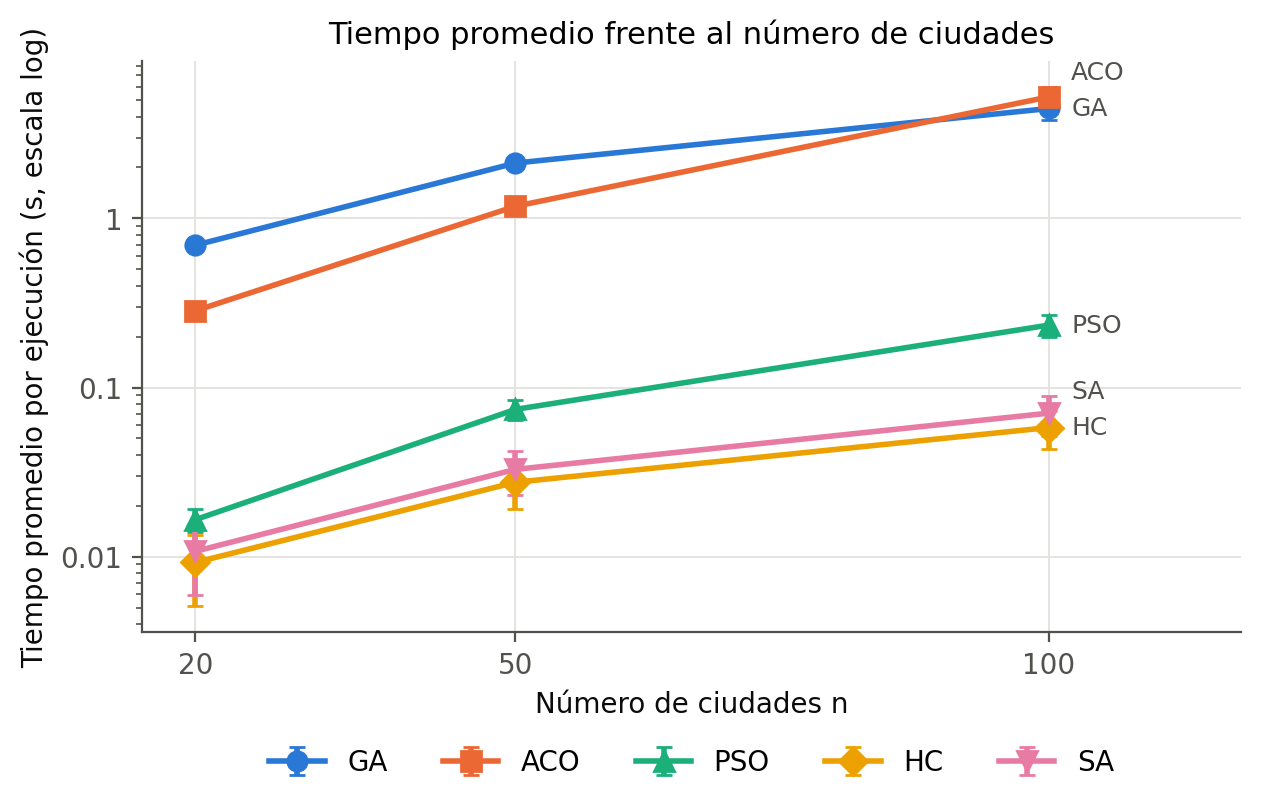
\includegraphics[width=0.49\linewidth]{fig3a_tiempo_vs_n.png}\hfill
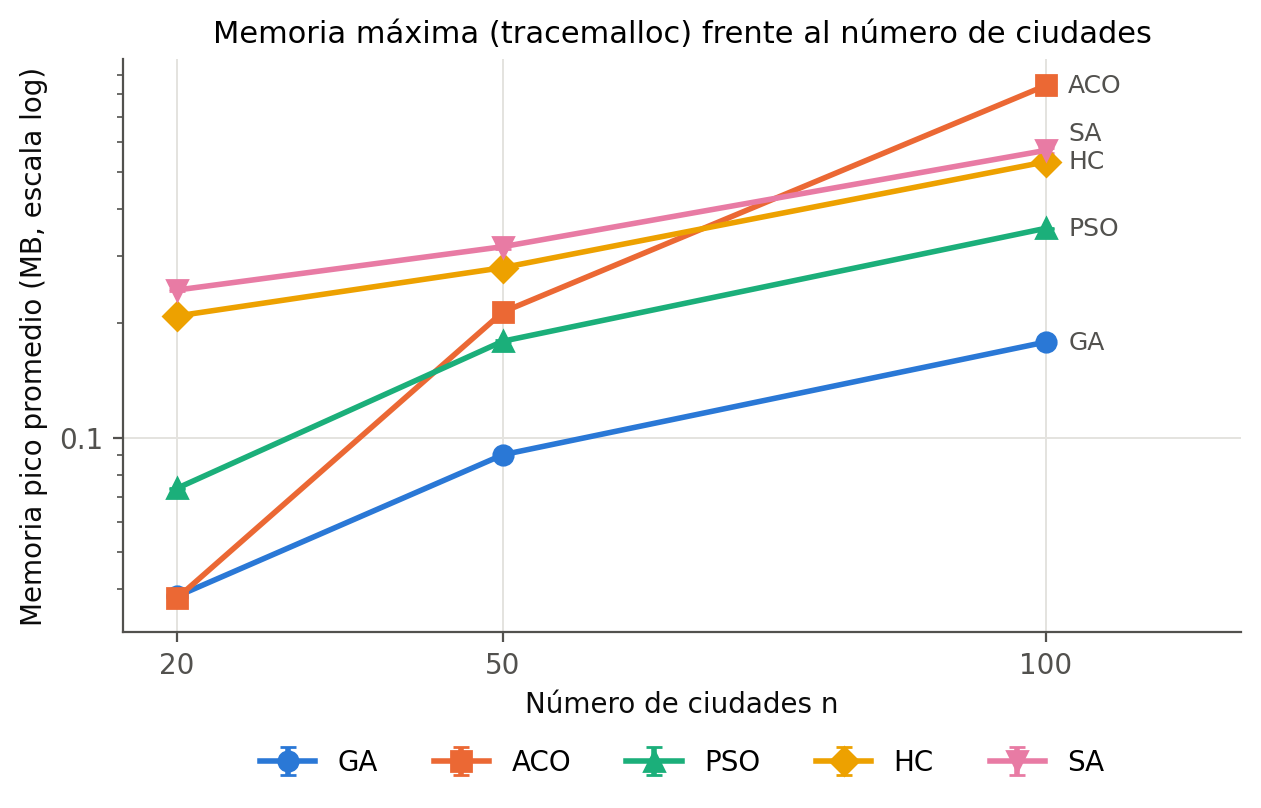
\includegraphics[width=0.49\linewidth]{fig3b_memoria_vs_n.png}
\caption{(a) Tiempo promedio por ejecución y (b) memoria pico promedio (\texttt{tracemalloc}) frente a $n$, ambos en escala logarítmica.
Barras: $\pm$ una desviación estándar. Cada punto promedia 150 corridas (tiempo) o 25 corridas (memoria).}
\end{figure}

\begin{table}[H]\centering\small
\begin{tabular}{clrrrrrr}
\toprule
$n$ & Alg. & tiempo (s) & ms/1000 FEs & memoria (MB) & éxito (\%) & FEs al 1\% (med.) & llegaron \\
\midrule
20 & GA & 0{,}694 & 69{,}4 & 0{,}038 & 36{,}0 & 3\,488 & 54/150 \\
 & ACO & 0{,}284 & 28{,}4 & 0{,}038 & 99{,}3 & 242 & 149/150 \\
 & PSO & 0{,}017 & 1{,}7 & 0{,}074 & 0{,}7 & 3\,417 & 1/150 \\
 & HC & 0{,}009 & 0{,}9 & 0{,}209 & 73{,}3 & 3\,076 & 110/150 \\
 & SA & 0{,}011 & 1{,}1 & 0{,}245 & 70{,}7 & 3\,324 & 106/150 \\
\midrule
50 & GA & 2{,}124 & 70{,}8 & 0{,}090 & 2{,}0 & 22\,710 & 3/150 \\
 & ACO & 1{,}179 & 39{,}3 & 0{,}214 & 66{,}0 & 7\,713 & 99/150 \\
 & PSO & 0{,}074 & 2{,}5 & 0{,}180 & 0{,}0 & -- & 0/150 \\
 & HC & 0{,}028 & 0{,}9 & 0{,}280 & 2{,}7 & 11\,162 & 4/150 \\
 & SA & 0{,}033 & 1{,}1 & 0{,}318 & 16{,}0 & 18\,560 & 24/150 \\
\midrule
100 & GA & 4{,}463 & 74{,}4 & 0{,}179 & 0{,}0 & -- & 0/150 \\
 & ACO & 5{,}228 & 87{,}1 & 0{,}845 & 17{,}3 & 34\,784 & 26/150 \\
 & PSO & 0{,}234 & 3{,}9 & 0{,}356 & 0{,}0 & -- & 0/150 \\
 & HC & 0{,}058 & 1{,}0 & 0{,}532 & 0{,}0 & -- & 0/150 \\
 & SA & 0{,}071 & 1{,}2 & 0{,}570 & 4{,}0 & 53\,696 & 6/150 \\
\bottomrule
\end{tabular}

\caption{Eficiencia por tamaño. ``ms/1000 FEs'': milisegundos por cada mil evaluaciones. ``FEs al 1\,\%'': mediana de las evaluaciones que tardó
en llegar a error $\le1\,\%$, calculada \emph{solo entre las corridas que llegaron}; ``llegaron'' dice cuántas de las 150 lo lograron.}
\end{table}

\subsection{Lectura de los resultados}
\begin{itemize}
\item \textbf{Más rápidos: HC y SA}, con diferencia. Con $n=100$ una corrida completa tarda 0{,}06--0{,}07\,s, unas \textbf{80 veces menos} que ACO (5{,}2\,s)
      o GA (4{,}5\,s). Y su costo por cada 1000 evaluaciones casi no cambia con $n$ ($\approx0{,}9$--$1{,}2$\,ms): la fórmula $\Delta$ del 2-opt es $O(1)$.
\item \textbf{ACO es el que peor escala en tiempo}: sus ms/1000 FEs pasan de 28 ($n=20$) a 87 ($n=100$). Construir \emph{una} ruta exige $n$ pasos y en cada paso
      mirar hasta $n$ candidatas: $O(n^2)$ por evaluación.
\item \textbf{GA es lento pero estable en costo por FE} ($\approx70$\,ms/1000): su costo está dominado por el trabajo en Python por cada hijo (torneos, cruce OX),
      no por $n$. \textbf{PSO} es rapidísimo porque todo el enjambre se actualiza con operaciones de matrices de NumPy.
\item \textbf{Memoria}: ACO crece más rápido ($\times22$ de $n=20$ a $n=100$) porque guarda matrices $n\times n$ (feromona, atractivo) y $m=n$ rutas.
      GA y PSO crecen $\approx\times5$ (lineal: población $\times\,n$). HC y SA empiezan más altos porque su vecindad guarda una copia de la matriz de distancias
      como listas de Python (acceso más rápido, más memoria), y bloques de números aleatorios pre-generados.
      Todas las cifras están por debajo de 1\,MB: para estos tamaños la memoria no es un problema real.
\end{itemize}

\begin{mate}[{Complejidad por evaluación (lo que explica las pendientes)}]
\begin{center}
\begin{tabular}{>{\raggedright}p{1.4cm}>{\raggedright}p{5.9cm}>{\raggedright\arraybackslash}p{5.9cm}}
\toprule
Algoritmo & Tiempo por FE & Memoria \\
\midrule
HC, SA & $O(1)$ con $\Delta$ ($+O(n)$ al aceptar, por invertir el tramo) & $O(n^2)$ (copia de $D$) o $O(n)$ si se calcula $d_{ij}$ al vuelo\\
GA & $O(n)$ (cruce, mutación, costo) & $O(P\,n)$\\
PSO & $O(n\log n)$ (ordenar las claves) & $O(S\,n)$\\
ACO & $O(n)$ por paso $\times\ n$ pasos $=O(n^2)$ & $O(n^2)$ (feromona) $+\,O(m\,n)$\\
\bottomrule
\end{tabular}
\end{center}
\end{mate}

\subsection{¿Cuál escala mejor? (inciso d)}
Depende de qué entendamos por ``escalar'', y por eso hay que mirar las dos cosas juntas (figura~\ref{fig:errorn}):
\begin{itemize}
\item \textbf{En costo computacional}, escalan mejor \textbf{HC y SA}: tiempo por FE constante y memoria pequeña.
\item \textbf{En calidad}, escala mejor \textbf{ACO}: su error mediano pasa de 0\,\% a 0{,}7\,\% y a 2{,}7\,\%; el de SA de 0 a 2{,}5 y a 4{,}6\,\%;
      el de HC de 0 a 4{,}4 y a 9{,}0\,\%; el de GA de 1{,}6 a 6{,}6 y a 14{,}9\,\%; y PSO se dispara de 23 a 228\,\%.
\item Tasa de éxito ($\le1\,\%$): ACO 99\,\%\,/\,66\,\%\,/\,17\,\%, SA 71/16/4\,\%, HC 73/3/0\,\%, GA 36/2/0\,\%, PSO $\approx0$.
      Con $n=100$ \emph{solo ACO y SA} llegan alguna vez al umbral.
\end{itemize}

\begin{figure}[H]\centering
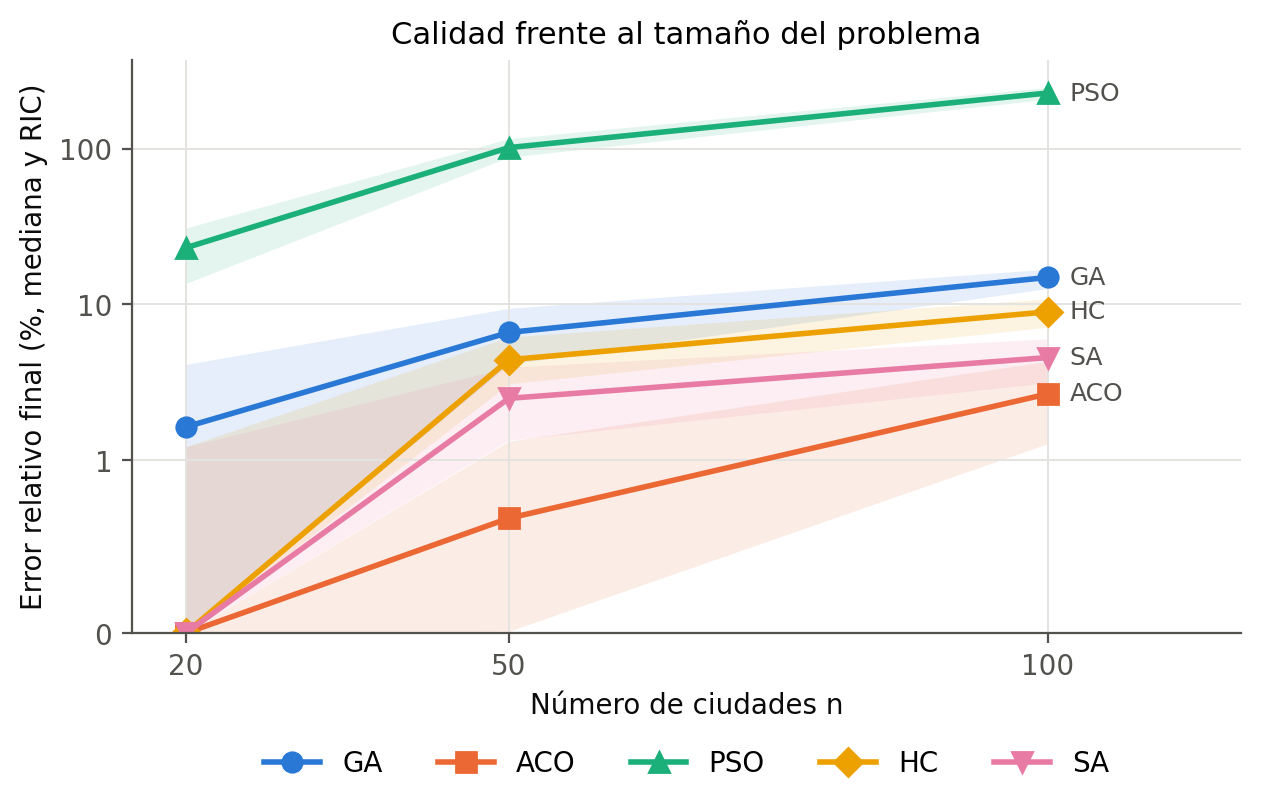
\includegraphics[width=0.62\linewidth]{fig3d_error_vs_n.png}
\caption{Error relativo final frente a $n$ (línea: mediana; banda: rango intercuartílico). Escala simétrica logarítmica: lineal entre 0 y 1\,\%, logarítmica arriba.}
\label{fig:errorn}
\end{figure}

\begin{porque}[{Rapidez no es calidad}]
HC termina una corrida con $n=100$ en 0{,}06\,s, pero su ruta es $\approx9\,\%$ más larga que la mejor conocida; ACO tarda 80 veces más y queda a $\approx2{,}7\,\%$.
PSO es el tercero más rápido y el peor en calidad por lejos. Terminar antes no significa haber encontrado algo bueno: por eso el taller pide
reportar tiempo \emph{y} calidad, y por eso el presupuesto se mide en \FEs\ y no en segundos.
\end{porque}

% =====================================================================
\section{Punto 4: rendimiento, convergencia y estabilidad}\label{sec:p4}
% =====================================================================

\subsection{(a) Curvas de convergencia promedio con banda de variabilidad}

\begin{idea}
Una curva de convergencia es la ``película'' de la búsqueda: en el eje $x$ el presupuesto gastado y en el eje $y$ la mejor ruta encontrada \emph{hasta ese momento}.
Siempre baja o se queda plana (nunca sube, porque es la mejor histórica). Una curva que baja rápido = algoritmo que encuentra cosas buenas con pocas evaluaciones.
\end{idea}

\begin{porque}[{¿Por qué interpolar en puntos comunes de \FEs?}]
Cada corrida registra su historial solo cuando mejora, en momentos distintos (una mejora en la evaluación 137, otra en la 212\dots).
Si promediáramos ``la mejora número 5'' de cada corrida estaríamos mezclando momentos distintos. Por eso cada curva se evalúa en los
\emph{mismos} 50 puntos del presupuesto (del 1\,\% al 100\,\%, espaciados logarítmicamente) y recién ahí se promedia.
Como la curva es escalonada, su valor en el punto $t$ es el último mejor costo registrado con $\text{FEs}\le t$
(función \texttt{mejor\_en\_puntos} en \archivo{src/tsp.py}). Además se grafica el \textbf{error} (\%) y no el costo, para poder promediar instancias
de longitudes distintas.
\end{porque}

\begin{figure}[H]\centering
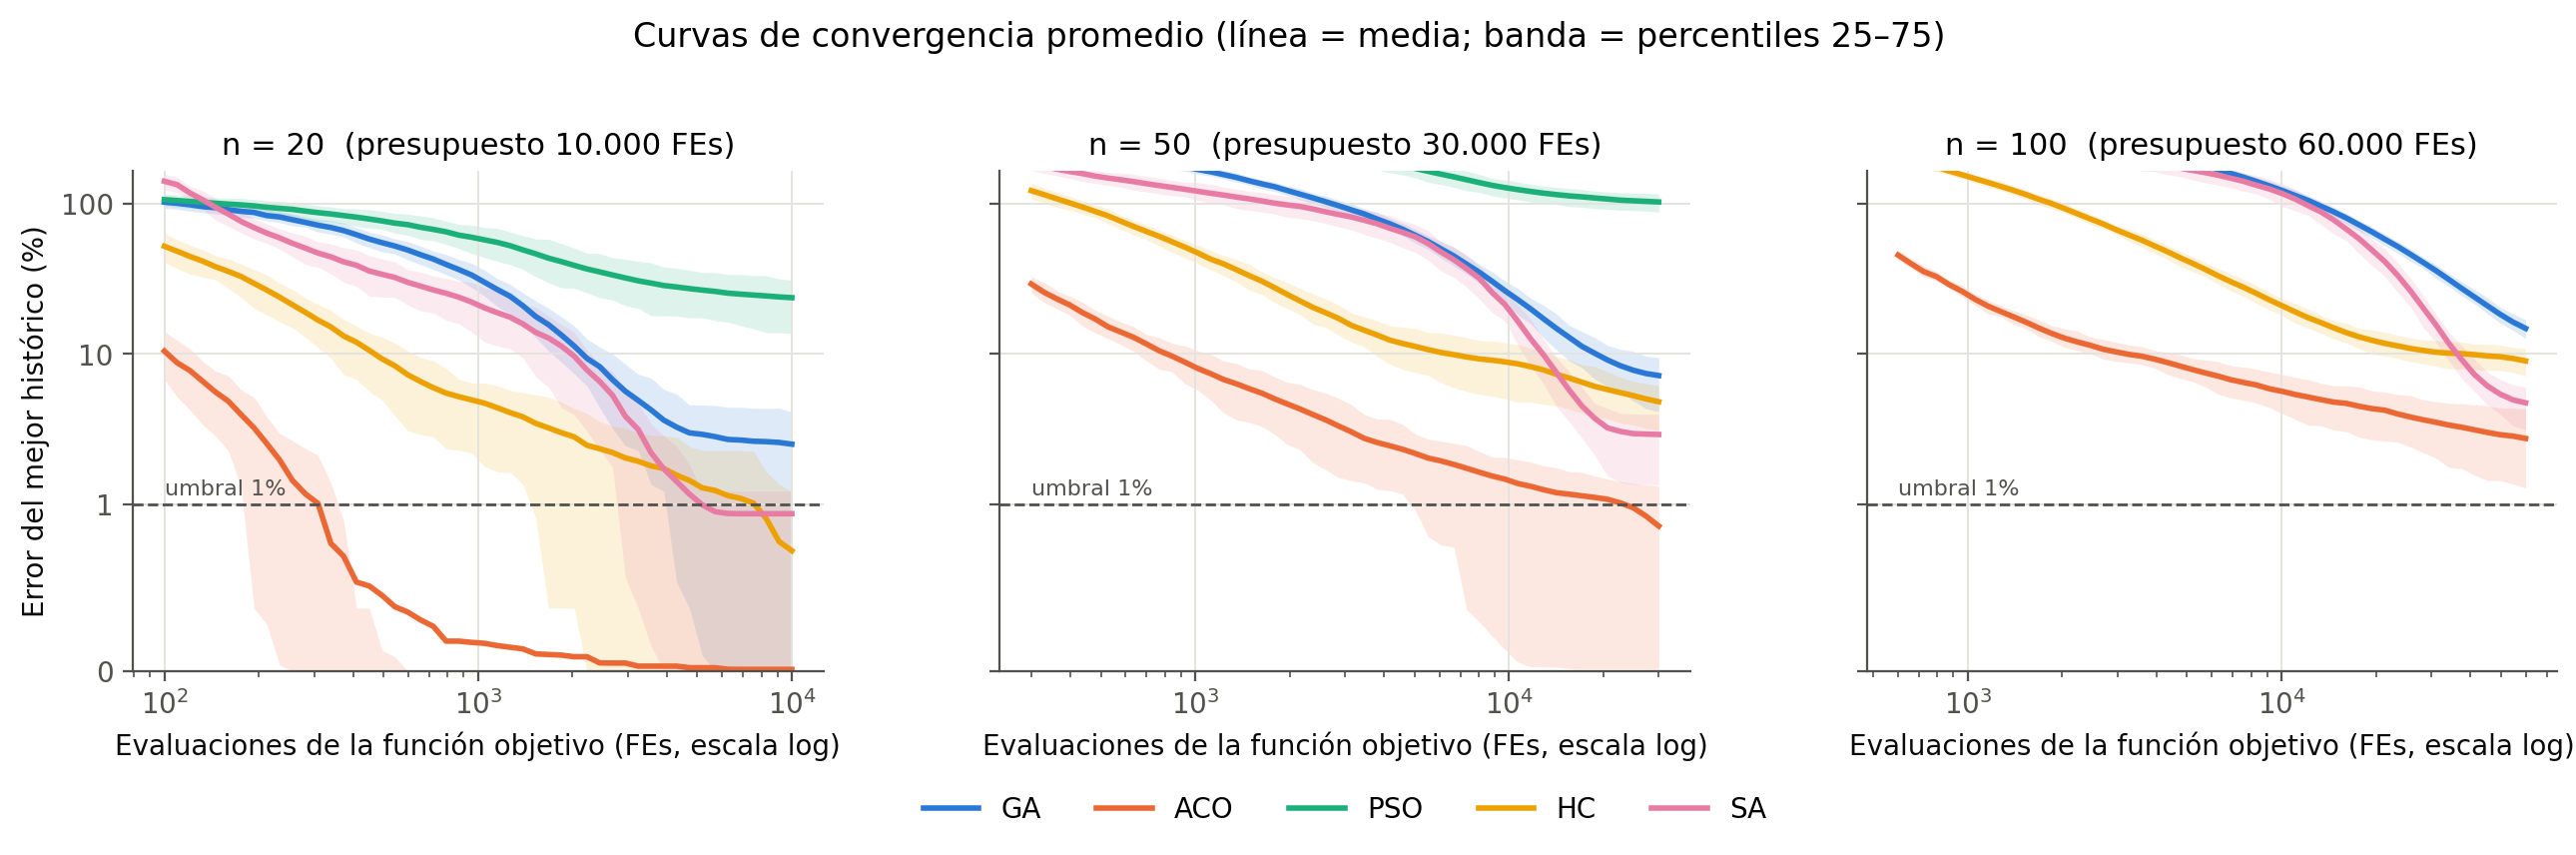
\includegraphics[width=\linewidth]{fig4a_convergencia.png}
\caption{Curvas de convergencia: error del mejor histórico frente a las \FEs\ (ambos ejes logarítmicos; el eje $y$ es lineal entre 0 y 1\,\%).
Línea: media de 150 corridas; banda: percentiles 25--75. Línea discontinua: umbral de 1\,\%.}
\end{figure}

\textbf{Qué se ve:}
\begin{itemize}
\item \textbf{ACO arranca muchísimo mejor}: su primera ruta ya es buena porque la visibilidad $1/d_{ij}$ la hace ``ir a la ciudad cercana''. Con solo el 10\,\% del presupuesto
      su error medio es 0{,}2\,\% ($n=20$), 3{,}3\,\% ($n=50$) y 7{,}5\,\% ($n=100$).
\item \textbf{HC baja rápido al principio} (explota desde el primer momento) y luego se aplana: se atasca en óptimos locales.
\item \textbf{SA tiene la forma típica en ``S''}: al principio, caliente, acepta muchos empeoramientos y casi no mejora (se ve peor que HC);
      al final, cuando se enfría, cae en picada y \textbf{adelanta a HC} en $n=50$ y $n=100$. Es la exploración ``pagando'' al final.
\item \textbf{GA sigue bajando al final} (su mejor solución aparece, en mediana, en el 98\,\% del presupuesto con $n=100$): no ha convergido; con más presupuesto mejoraría.
\item \textbf{PSO casi no baja}: el enjambre se estanca por la codificación de claves aleatorias.
\end{itemize}

\subsection{(b) Diagramas de caja del error relativo final}
\begin{figure}[H]\centering
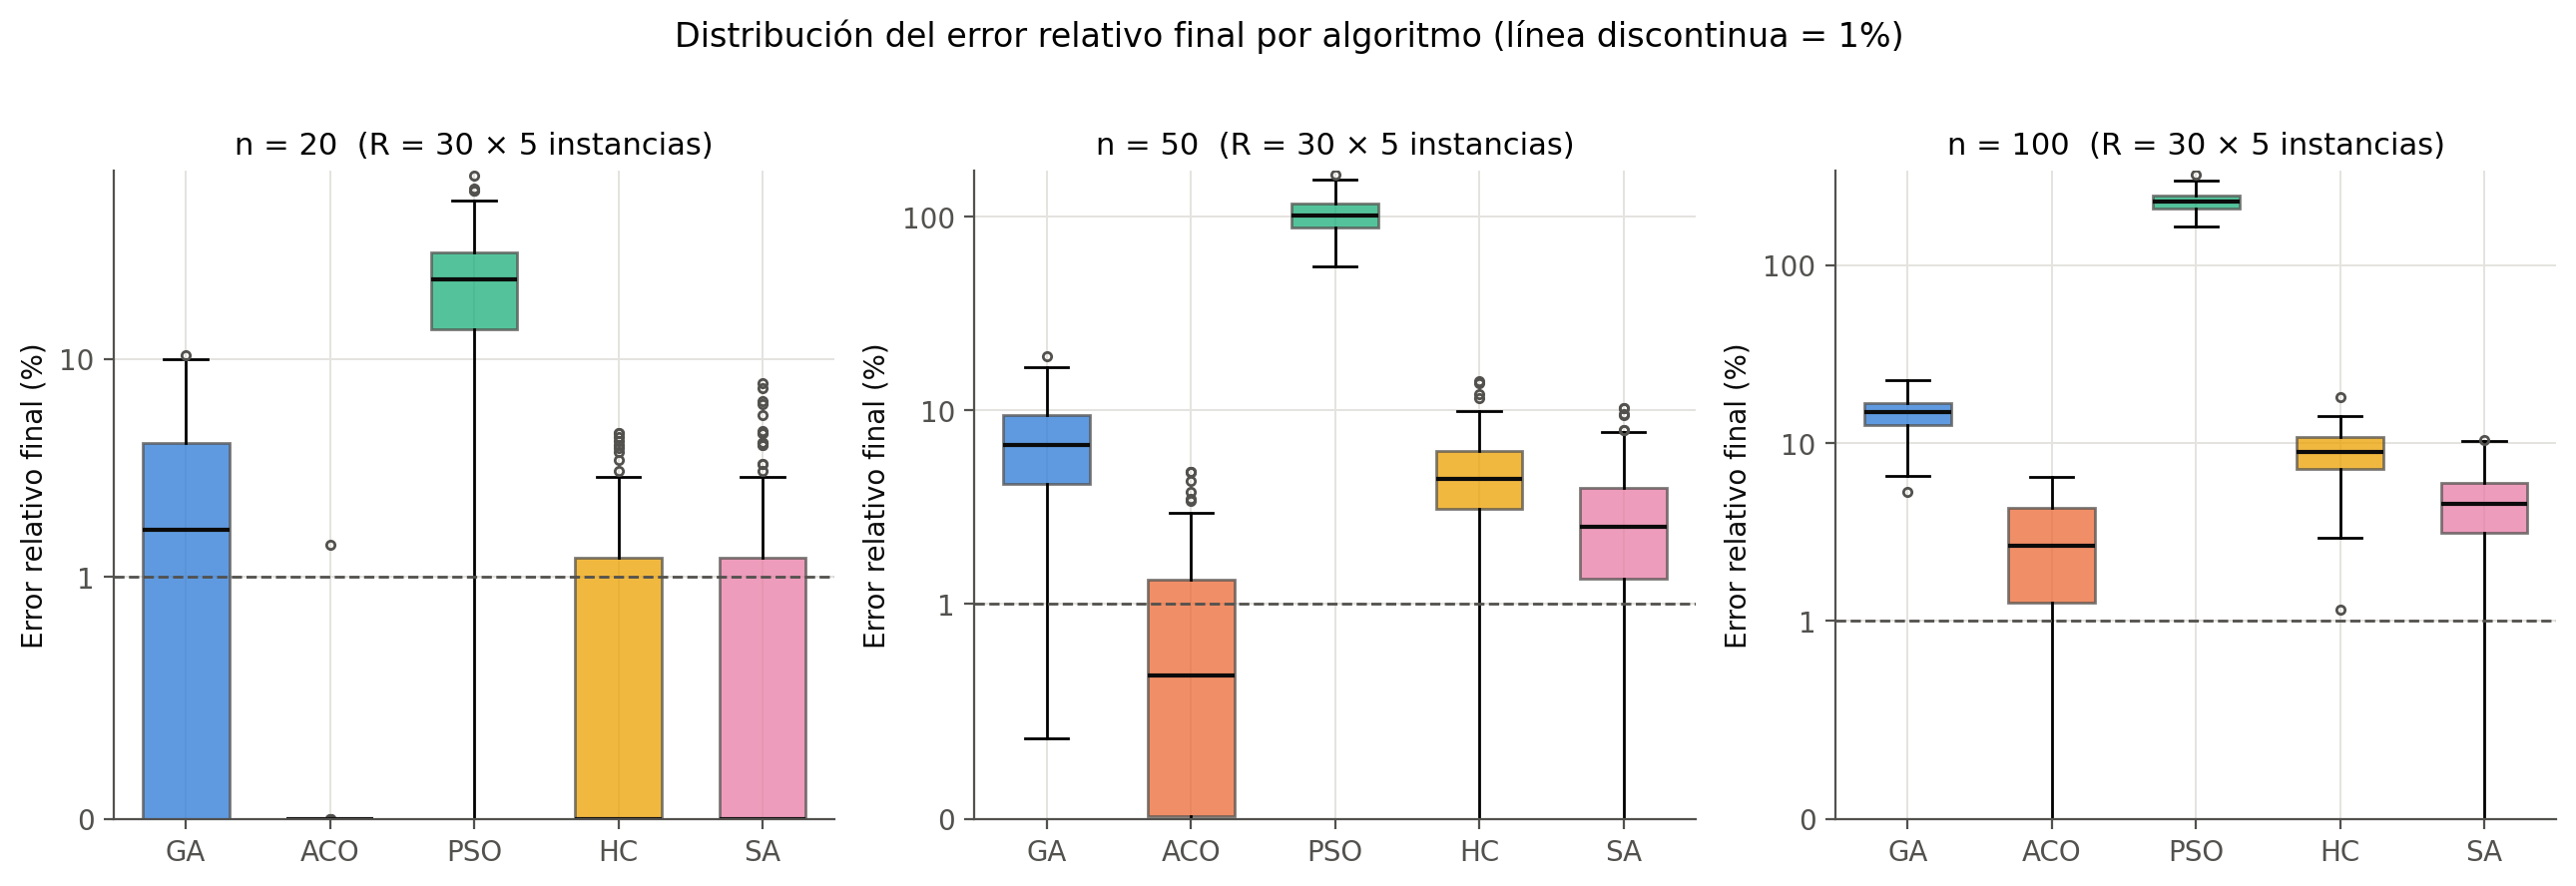
\includegraphics[width=\linewidth]{fig4b_cajas_error.png}
\caption{Error relativo final de las 150 corridas por algoritmo y tamaño (5 instancias $\times$ 30 repeticiones). Caja: RIC; línea negra: mediana;
bigotes: $1{,}5\cdot$RIC; puntos: atípicos. Escala lineal entre 0 y 1\,\% y logarítmica arriba.}
\end{figure}
La caja de ACO es la más baja en los tres tamaños; con $n=20$ es prácticamente una línea en 0 (casi todas las corridas encuentran la mejor ruta conocida).
La de PSO está uno o dos órdenes de magnitud por encima. Entre HC y SA: con $n=20$ son casi iguales; con $n=50$ y $n=100$ la caja de SA está claramente más abajo.

\subsection{(c) Tabla de rendimiento}
\begin{table}[H]\centering\small
\begin{tabular}{clrrrrrrr}
\toprule
$n$ & Alg. & mejor & media & mediana & desv.$^\dagger$ & RIC & éxito (\%) & mejora (\%) \\
\midrule
20 & GA & 0{,}00 & 2{,}51 & 1{,}63 & 2{,}14 & 4{,}12 & 36{,}0 & 61{,}7 \\
 & ACO & 0{,}00 & 0{,}01 & 0{,}00 & 0{,}05 & 0{,}00 & 99{,}3 & 40{,}9 \\
 & PSO & 0{,}00 & 23{,}67 & 23{,}10 & 13{,}07 & 17{,}30 & 0{,}7 & 53{,}8 \\
 & HC & 0{,}00 & 0{,}72 & 0{,}00 & 0{,}89 & 1{,}22 & 73{,}3 & 62{,}3 \\
 & SA & 0{,}00 & 0{,}94 & 0{,}00 & 0{,}98 & 1{,}22 & 70{,}7 & 62{,}2 \\
\midrule
50 & GA & 0{,}37 & 7{,}17 & 6{,}61 & 3{,}70 & 5{,}31 & 2{,}0 & 76{,}3 \\
 & ACO & 0{,}00 & 0{,}87 & 0{,}66 & 0{,}62 & 1{,}31 & 66{,}0 & 55{,}8 \\
 & PSO & 55{,}13 & 102{,}71 & 101{,}72 & 19{,}69 & 27{,}99 & 0{,}0 & 55{,}5 \\
 & HC & 0{,}00 & 4{,}80 & 4{,}41 & 2{,}36 & 3{,}09 & 2{,}7 & 76{,}8 \\
 & SA & 0{,}00 & 2{,}91 & 2{,}50 & 2{,}06 & 2{,}61 & 16{,}0 & 77{,}2 \\
\midrule
100 & GA & 5{,}29 & 14{,}78 & 14{,}91 & 3{,}30 & 4{,}22 & 0{,}0 & 82{,}2 \\
 & ACO & 0{,}00 & 2{,}73 & 2{,}66 & 0{,}89 & 3{,}04 & 17{,}3 & 63{,}5 \\
 & PSO & 165{,}26 & 230{,}27 & 228{,}01 & 24{,}07 & 39{,}56 & 0{,}0 & 48{,}6 \\
 & HC & 1{,}17 & 8{,}98 & 8{,}97 & 2{,}52 & 3{,}72 & 0{,}0 & 83{,}1 \\
 & SA & 0{,}00 & 4{,}72 & 4{,}56 & 2{,}19 & 2{,}87 & 4{,}0 & 83{,}8 \\
\bottomrule
\end{tabular}

\caption{Error relativo final (\%) respecto a $f^\ast$ sobre las 150 corridas de cada tamaño. $^\dagger$Desviación estándar calculada \emph{dentro} de cada instancia y promediada
(así no se mezcla la variación entre instancias con la del algoritmo). Éxito: \% de corridas con error $\le1\,\%$. Mejora: $100(f_{\text{inicial}}-f_r)/f_{\text{inicial}}$.}
\end{table}

\begin{porque}[{¿Por qué la tabla principal usa el error y no el costo?}]
El costo de una ruta en la instancia 0 no se puede promediar con el de la instancia 3: son mapas distintos. El error relativo pone todo en la misma escala
(``qué tan lejos del mejor conocido, en \%''). Aun así, el taller pide mejor, media, mediana y desviación \emph{del costo}; están por instancia en
\archivo{resultados/tabla\_rendimiento\_por\_instancia.csv}. Aquí va la instancia 0 como ejemplo:
\end{porque}

\begin{table}[H]\centering\small
\begin{tabular}{clrrrr}
\toprule
$n$ & Alg. & mejor & media & mediana & desv. \\
\midrule
20 & GA & 426{,}62 & 449{,}34 & 449{,}76 & 10{,}35 \\
 & ACO & 426{,}62 & 426{,}62 & 426{,}62 & 0{,}00 \\
 & PSO & 453{,}08 & 517{,}45 & 508{,}32 & 45{,}92 \\
 & HC & 426{,}62 & 435{,}51 & 438{,}52 & 6{,}86 \\
 & SA & 426{,}62 & 439{,}37 & 438{,}82 & 9{,}86 \\
\midrule
50 & GA & 549{,}17 & 579{,}16 & 576{,}58 & 20{,}77 \\
 & ACO & 543{,}14 & 547{,}78 & 548{,}04 & 1{,}92 \\
 & PSO & 886{,}86 & 1\,094{,}18 & 1\,087{,}42 & 110{,}04 \\
 & HC & 549{,}71 & 567{,}60 & 565{,}32 & 12{,}81 \\
 & SA & 547{,}74 & 556{,}62 & 551{,}58 & 9{,}27 \\
\midrule
100 & GA & 879{,}36 & 949{,}65 & 953{,}36 & 25{,}35 \\
 & ACO & 837{,}26 & 852{,}18 & 851{,}89 & 8{,}72 \\
 & PSO & 2\,313{,}43 & 2\,608{,}71 & 2\,541{,}44 & 176{,}22 \\
 & HC & 844{,}95 & 900{,}43 & 901{,}58 & 21{,}17 \\
 & SA & 848{,}68 & 873{,}53 & 873{,}65 & 15{,}28 \\
\bottomrule
\end{tabular}

\caption{Costo final (longitud de la ruta) en la instancia 0 de cada tamaño, 30 repeticiones.}
\end{table}

\textbf{Ojo con la columna ``mejora''}: ACO tiene la mejora \emph{más baja} (41--64\,\%) siendo el mejor. No es contradicción: su primera ruta ya era buena, así que
``mejoró menos'' porque arrancó más cerca de la meta. Por eso la mejora no sirve sola para comparar algoritmos que arrancan de formas distintas.

\subsection{(d) Rutas de los cinco métodos en la misma instancia}
\begin{figure}[H]\centering
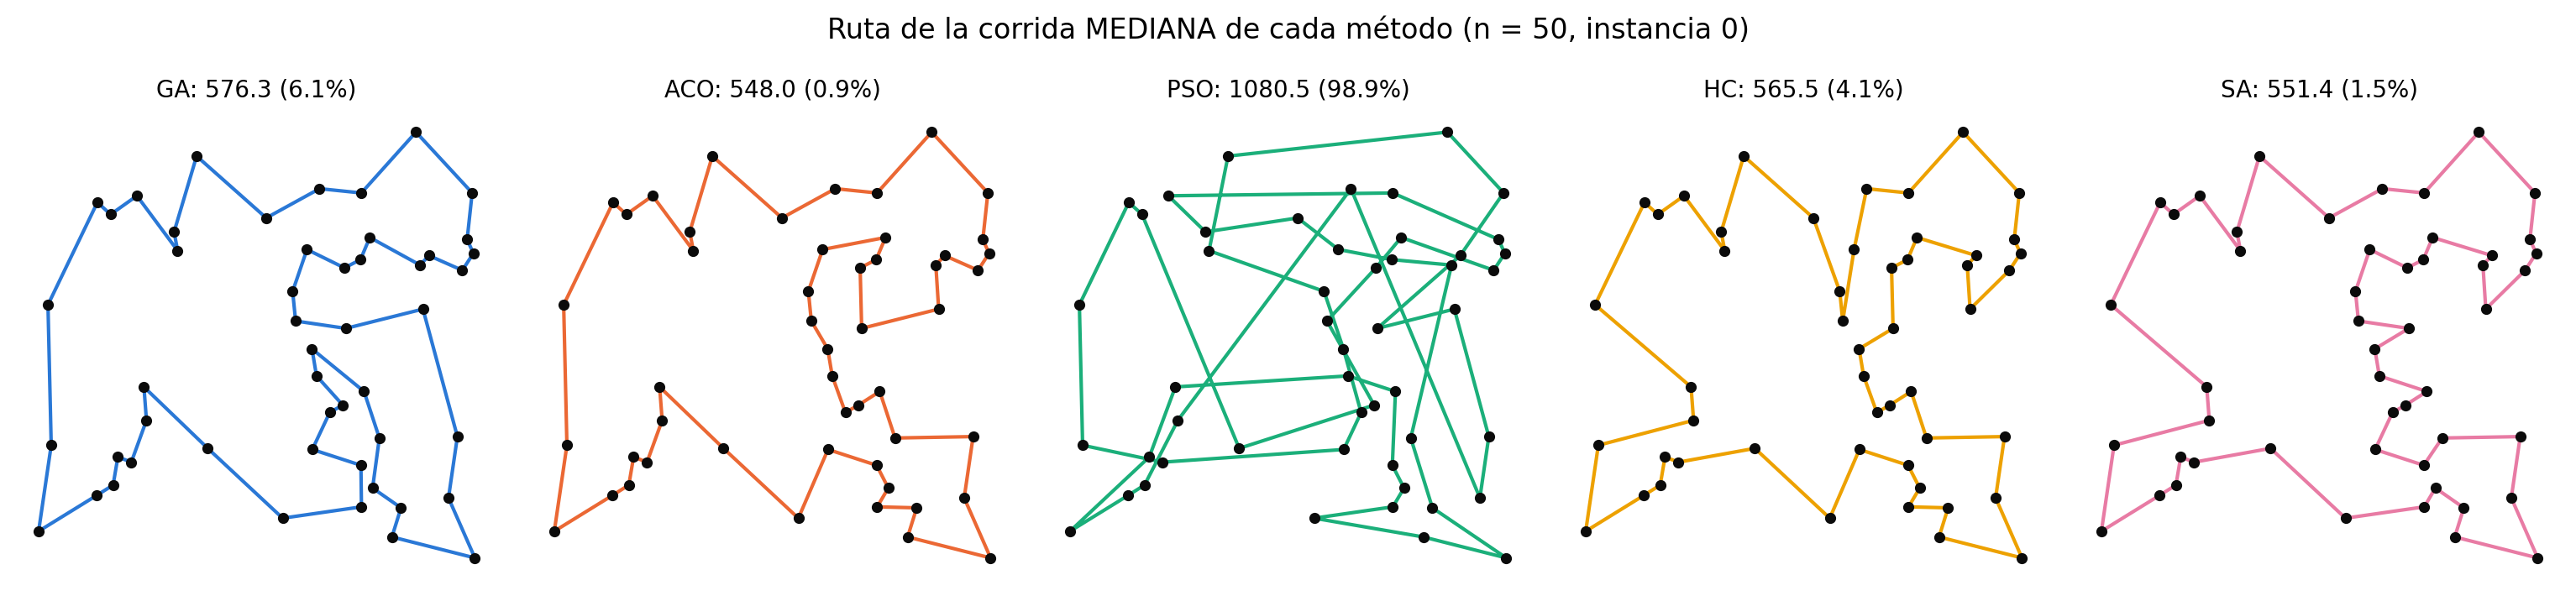
\includegraphics[width=\linewidth]{fig4d_rutas.png}
\caption{Ruta de la corrida \emph{mediana} (no la mejor) de cada método en la instancia 0 con $n=50$. Entre paréntesis, el error respecto a $f^\ast$.}
\end{figure}
Se escogió la corrida mediana y no la mejor porque la mejor es ``la foto más bonita'', no la típica. Fíjate: las rutas de ACO, SA y HC no tienen cruces (2-opt los elimina);
la de GA tiene zonas enredadas; la de PSO está llena de cruces: prácticamente no aprendió la geometría del problema.

\subsection{(e) Ranking por calidad, estabilidad y velocidad de convergencia}
Criterios:
\begin{itemize}
\item \textbf{Calidad}: rango promedio de Friedman ($\bar R$; 1 = siempre el mejor, 5 = siempre el peor).
\item \textbf{Estabilidad}: desviación estándar del error dentro de cada instancia, promediada (más pequeña = más estable).
\item \textbf{Velocidad}: área bajo la curva de error medio en el eje $\log(\text{FEs})$ (AUC). Un área pequeña significa que la curva bajó pronto.
\item \textbf{Global}: promedio de las tres posiciones.
\end{itemize}
\begin{table}[H]\centering\small
\begin{tabular}{clccccrrr}
\toprule
$n$ & Alg. & calidad & estab. & veloc. & global & $\bar R$ & desv. error & AUC \\
\midrule
20 & ACO & 1 & 1 & 1 & \textbf{1} & 1{,}84 & 0{,}05 & 2{,}5 \\
 & HC & 2 & 2 & 2 & \textbf{2} & 2{,}31 & 0{,}89 & 22{,}9 \\
 & SA & 3 & 3 & 3 & \textbf{3} & 2{,}58 & 0{,}98 & 64{,}2 \\
 & GA & 4 & 4 & 4 & \textbf{4} & 3{,}31 & 2{,}14 & 79{,}1 \\
 & PSO & 5 & 5 & 5 & \textbf{5} & 4{,}95 & 13{,}07 & 120{,}2 \\
\midrule
50 & ACO & 1 & 1 & 1 & \textbf{1} & 1{,}31 & 0{,}62 & 12{,}6 \\
 & SA & 2 & 2 & 3 & \textbf{2} & 2{,}17 & 2{,}06 & 157{,}7 \\
 & HC & 3 & 3 & 2 & \textbf{3} & 3{,}02 & 2{,}36 & 65{,}9 \\
 & GA & 4 & 4 & 4 & \textbf{4} & 3{,}50 & 3{,}70 & 208{,}0 \\
 & PSO & 5 & 5 & 5 & \textbf{5} & 5{,}00 & 19{,}69 & 389{,}0 \\
\midrule
100 & ACO & 1 & 1 & 1 & \textbf{1} & 1{,}26 & 0{,}89 & 22{,}1 \\
 & SA & 2 & 2 & 3 & \textbf{2} & 1{,}88 & 2{,}19 & 284{,}9 \\
 & HC & 3 & 3 & 2 & \textbf{3} & 2{,}93 & 2{,}52 & 120{,}9 \\
 & GA & 4 & 4 & 4 & \textbf{4} & 3{,}93 & 3{,}30 & 363{,}7 \\
 & PSO & 5 & 5 & 5 & \textbf{5} & 5{,}00 & 24{,}07 & 726{,}5 \\
\bottomrule
\end{tabular}

\caption{Ranking por tamaño (ordenado por la posición global).}
\end{table}
ACO es primero en los tres criterios y en los tres tamaños; PSO es último en todo. El orden intermedio cambia: con $n=20$ HC supera a SA; con $n=50$ y $n=100$
SA es segundo en calidad y estabilidad, aunque HC sigue siendo más rápido en converger (SA ``gasta'' la primera parte explorando).

% =====================================================================
\section{La estadística, explicada sin miedo}\label{sec:estadistica}
% =====================================================================
El taller advierte: \emph{``no es correcto concluir que un algoritmo es superior únicamente porque su media sea ligeramente menor''}.
Esta sección explica las herramientas para decir ``A es mejor que B'' con evidencia.

\subsection{Media, mediana, desviación y rango intercuartílico}
\begin{mate}
Para los resultados $x_1,\dots,x_R$ de las corridas:
\[
\bar x=\frac1R\sum_{r=1}^R x_r,\qquad s=\sqrt{\frac{1}{R-1}\sum_{r=1}^R (x_r-\bar x)^2},\qquad \text{RIC}=Q_3-Q_1 .
\]
La \textbf{mediana} es el valor del medio al ordenar los datos; $Q_1$ y $Q_3$ son los percentiles 25 y 75.
\end{mate}
\begin{idea}
Si en un grupo de 10 personas 9 ganan un millón y una gana mil millones, la \emph{media} dice que ``en promedio ganan 100 millones'', lo cual
no describe a nadie. La \emph{mediana} (un millón) sí. Con los algoritmos pasa lo mismo: una sola corrida muy mala sube la media, pero no la mediana.
Por eso el taller pide \textbf{mediana y RIC}: son \textbf{robustas} a valores extremos. El RIC es ``el ancho de la caja'' en un diagrama de caja:
entre $Q_1$ y $Q_3$ está la mitad central de las corridas.
\end{idea}

\subsection{¿Cómo se lee un diagrama de caja?}
\begin{center}
\begin{tikzpicture}[scale=1.0]
\draw[thick] (0,0)--(1.5,0); \draw[thick] (1.5,-0.4) rectangle (4.5,0.4); \draw[very thick] (2.6,-0.4)--(2.6,0.4);
\draw[thick] (4.5,0)--(6.5,0); \draw (0,-0.2)--(0,0.2); \draw (6.5,-0.2)--(6.5,0.2); \fill (7.6,0) circle (2pt);
\node[below,font=\small] at (0,-0.3) {mínimo*}; \node[above,font=\small] at (1.5,0.45) {$Q_1$};
\node[below,font=\small] at (2.6,-0.45) {mediana}; \node[above,font=\small] at (4.5,0.45) {$Q_3$};
\node[below,font=\small] at (6.5,-0.3) {máximo*}; \node[above,font=\small] at (7.6,0.1) {atípico};
\draw[decorate,decoration={brace,amplitude=4pt}] (1.5,0.9)--(4.5,0.9) node[midway,above=4pt,font=\small] {RIC (50\,\% central)};
\end{tikzpicture}\\[-0.2em]
{\footnotesize *los bigotes llegan hasta $1{,}5\cdot$RIC; lo que queda por fuera se dibuja como punto (atípico).}
\end{center}
Caja \textbf{baja} = buena calidad; caja \textbf{angosta} = algoritmo \textbf{estable} (da resultados parecidos siempre).

\subsection{Prueba de Friedman: ¿hay \emph{alguna} diferencia entre los cinco?}
\begin{idea}
Imagina 150 ``carreras'' (5 instancias $\times$ 30 repeticiones). En cada carrera participan los 5 algoritmos con la misma semilla y se les da
un puesto: 1.º (ruta más corta), 2.º, \dots, 5.º. Si todos fueran igual de buenos, en promedio cada uno quedaría de 3.º.
Friedman mide si los puestos promedio se alejan demasiado de 3 como para ser casualidad.
Usa puestos (rangos) y no los costos, así que no le importa que las instancias tengan escalas distintas ni que los datos no sean normales.
\end{idea}
\begin{mate}[{Estadístico de Friedman}]
Con $N$ bloques (carreras), $k$ algoritmos y $\bar R_j$ el rango promedio del algoritmo $j$:
\[
\chi^2_F=\frac{12N}{k(k+1)}\left[\sum_{j=1}^{k}\bar R_j^{\,2}-\frac{k(k+1)^2}{4}\right]\;\sim\;\chi^2_{k-1}\ \text{(aprox.)}
\]
\textbf{Hipótesis nula} $H_0$: todos los algoritmos rinden igual. Si el valor $p<\alpha=0{,}05$, se rechaza $H_0$.\\
\textbf{Tamaño del efecto} (W de Kendall): $W=\dfrac{\chi^2_F}{N(k-1)}\in[0,1]$. $W\approx0$: los puestos cambian al azar entre carreras;
$W\approx1$: el orden de llegada es \emph{siempre} el mismo.
\end{mate}
\begin{porque}[{¿Qué es el valor $p$?}]
Es la probabilidad de ver diferencias \emph{tan grandes o mayores} que las observadas \emph{si en realidad no hubiera ninguna diferencia}.
Un $p$ muy pequeño dice: ``sería rarísimo ver esto por pura suerte''. Ojo: $p$ pequeño no dice \emph{cuánto} mejor es uno que otro; para eso está el
tamaño del efecto. Con 150 bloques, hasta diferencias pequeñas dan $p$ diminutos: por eso siempre se reporta también la magnitud.
\end{porque}

\subsection{Post hoc: ¿\emph{quién} es diferente de quién?}
Friedman solo dice ``hay diferencias en algún lado''. Para saber entre qué pares, se comparan los $\binom{5}{2}=10$ pares con la
\textbf{prueba de rangos con signo de Wilcoxon} (para datos pareados: compara corrida contra corrida con la misma semilla).

\begin{mate}[{Corrección de Holm}]
Al hacer 10 pruebas, la probabilidad de encontrar \emph{al menos un} falso positivo crece mucho (si cada una tiene 5\,\% de riesgo, con 10 pruebas
el riesgo total puede llegar a $\approx40\,\%$). Holm lo corrige:
\begin{enumerate}
\item Ordena los $m$ valores $p$ de menor a mayor: $p_{(1)}\le p_{(2)}\le\dots\le p_{(m)}$.
\item Ajusta: $p^{\text{Holm}}_{(i)}=\max_{l\le i}\ \min\{1,\ (m-l+1)\,p_{(l)}\}$.
\item Declara significativo el par si $p^{\text{Holm}}<0{,}05$.
\end{enumerate}
\textbf{Ejemplo} con $m=3$: $p=(0{,}01;\ 0{,}04;\ 0{,}03)$. Ordenados: $0{,}01;\ 0{,}03;\ 0{,}04$. Ajustados: $3(0{,}01)=0{,}03$;\; $2(0{,}03)=0{,}06$;\;
$\max(0{,}06,\ 1\cdot0{,}04)=0{,}06$. Solo el primero sigue siendo significativo.
\end{mate}
\begin{codigo}
\archivo{experimentos/analizar\_resultados.py}: \texttt{stats.friedmanchisquare}, \texttt{stats.wilcoxon} y la función \texttt{holm()}
escrita a mano (para que veas que no es magia). El tamaño del efecto por par es la \textbf{correlación biserial de rangos}
$r=\frac{\sum R^+-\sum R^-}{\sum R}\in[-1,1]$: negativo = A suele dar rutas más cortas que B; $|r|$ cerca de 1 = casi siempre.
\end{codigo}

\subsection{Resultados de las pruebas}
\begin{table}[H]\centering\small
\begin{tabular}{rrrrrrrrr}
\toprule
$n$ & $\chi^2_F$ & $p$ & $W$ & $\bar R$ GA & $\bar R$ ACO & $\bar R$ PSO & $\bar R$ HC & $\bar R$ SA \\
\midrule
20 & 379{,}6 & $<10^{-16}$ & 0{,}633 & 3{,}31 & 1{,}84 & 4{,}95 & 2{,}31 & 2{,}58 \\
\midrule
50 & 467{,}4 & $<10^{-16}$ & 0{,}779 & 3{,}50 & 1{,}31 & 5{,}00 & 3{,}02 & 2{,}17 \\
\midrule
100 & 549{,}5 & $<10^{-16}$ & 0{,}916 & 3{,}93 & 1{,}26 & 5{,}00 & 2{,}93 & 1{,}88 \\
\bottomrule
\end{tabular}

\caption{Prueba de Friedman por tamaño ($N=150$ bloques = 5 instancias $\times$ 30 repeticiones, $k=5$ algoritmos) y rangos promedio $\bar R$ (1 = mejor).}
\end{table}

En los tres tamaños $p<10^{-16}$: se rechaza que los cinco rindan igual. Más interesante es el \textbf{tamaño del efecto}: $W$ sube de 0{,}63 a 0{,}78 y a 0{,}92.
Es decir, \textbf{a medida que el problema crece, el orden entre algoritmos se vuelve casi fijo}: con $n=100$ casi todas las carreras terminan en el mismo orden
(ACO, SA, HC, GA, PSO).

\begin{table}[H]\centering\small
\begin{tabular}{llll}
\toprule
Par & $n=20$ & $n=50$ & $n=100$ \\
\midrule
GA vs ACO & ACO (0{,}88; $<10^{-4}$) & ACO (0{,}99; $<10^{-4}$) & ACO (1{,}00; $<10^{-4}$) \\
GA vs PSO & GA ($-$0{,}99; $<10^{-4}$) & GA ($-$1{,}00; $<10^{-4}$) & GA ($-$1{,}00; $<10^{-4}$) \\
GA vs HC & HC (0{,}70; $<10^{-4}$) & HC (0{,}54; $<10^{-4}$) & HC (0{,}96; $<10^{-4}$) \\
GA vs SA & SA (0{,}63; $<10^{-4}$) & SA (0{,}85; $<10^{-4}$) & SA (1{,}00; $<10^{-4}$) \\
ACO vs PSO & ACO ($-$1{,}00; $<10^{-4}$) & ACO ($-$1{,}00; $<10^{-4}$) & ACO ($-$1{,}00; $<10^{-4}$) \\
ACO vs HC & ACO ($-$0{,}51; $<10^{-4}$) & ACO ($-$0{,}96; $<10^{-4}$) & ACO ($-$1{,}00; $<10^{-4}$) \\
ACO vs SA & ACO ($-$0{,}63; $<10^{-4}$) & ACO ($-$0{,}77; $<10^{-4}$) & ACO ($-$0{,}66; $<10^{-4}$) \\
PSO vs HC & HC (1{,}00; $<10^{-4}$) & HC (1{,}00; $<10^{-4}$) & HC (1{,}00; $<10^{-4}$) \\
PSO vs SA & SA (1{,}00; $<10^{-4}$) & SA (1{,}00; $<10^{-4}$) & SA (1{,}00; $<10^{-4}$) \\
HC vs SA & HC ($-$0{,}21; 0{,}0258) & SA (0{,}65; $<10^{-4}$) & SA (0{,}92; $<10^{-4}$) \\
\bottomrule
\end{tabular}

\caption{Post hoc: Wilcoxon pareado con corrección de Holm (10 pares por tamaño). Cada celda: ganador (biserial de rangos; $p$ ajustado).
Biserial positivo: gana B; negativo: gana A. Todas las diferencias son significativas con $\alpha=0{,}05$.}
\end{table}

\textbf{Cómo leer un caso:} ``HC vs SA, $n=20$: HC ($-0{,}21$; 0{,}026)''. HC gana, pero el efecto es \emph{pequeño} ($|r|=0{,}21$) y el $p$ no es tan extremo:
son casi equivalentes con 20 ciudades. En cambio, ``HC vs SA, $n=100$: SA (0{,}92)'' significa que SA da una ruta más corta que HC en prácticamente
todas las corridas emparejadas. \textbf{Esto es exactamente lo que el taller pide}: no basta con que la media sea menor; hay que ver si la diferencia es
consistente (Wilcoxon + Holm) y de qué tamaño es (biserial, $W$).

% =====================================================================
\section{Punto 5: análisis crítico y conclusiones}\label{sec:p5}
% =====================================================================
Cada respuesta cita la evidencia (tabla o figura) que la sostiene. Así se debe escribir en el informe: \emph{afirmación + número + de dónde sale}.

\begin{respuesta}[{1. ¿Qué algoritmo obtuvo las rutas de menor costo y cuál fue el más estable?}]
\textbf{ACO en ambos casos, en los tres tamaños.} Error mediano 0{,}00 / 0{,}66 / 2{,}66\,\% para $n=20/50/100$ (tabla de rendimiento), rango de Friedman
1{,}84 / 1{,}31 / 1{,}26, y gana todas sus comparaciones pareadas con $p<10^{-4}$. También tiene la menor desviación dentro de cada instancia
(0{,}05 / 0{,}62 / 0{,}89 puntos de error) y la caja más angosta en la figura de cajas.
\end{respuesta}

\begin{respuesta}[{2. ¿Cuál alcanzó buenas soluciones usando menos evaluaciones?}]
\textbf{ACO.} Con $n=20$ llega al 1\,\% en una mediana de 242 \FEs\ (2{,}4\,\% del presupuesto), frente a unas 3100--3500 de HC, SA y GA.
Con $n=50$ necesita $\approx$7700 \FEs\ y lo logra en 99 de 150 corridas (HC: 4; GA: 3). Con $n=100$ es el único que llega con cierta frecuencia (26 de 150; SA: 6).
Si ``buena'' se entiende como ``bastante buena muy pronto'', \textbf{HC} es segundo: su curva baja más rápido que la de SA y GA al inicio.
\end{respuesta}

\begin{respuesta}[{3. ¿Cuál tuvo menor tiempo y menor memoria? ¿Coincide con el de mejor calidad?}]
\textbf{Tiempo: HC} (0{,}009 / 0{,}028 / 0{,}058\,s), seguido muy de cerca por SA. \textbf{Memoria: GA} (0{,}04 / 0{,}09 / 0{,}18\,MB; empatado con ACO en $n=20$).
\textbf{No coincide} con el de mejor calidad: ACO es el \emph{más lento} con $n=100$ (5{,}2\,s, $\approx90$ veces HC) y el que \emph{más memoria} usa (0{,}85\,MB).
Hay un intercambio (\emph{trade-off}) claro entre calidad y costo computacional.
\end{respuesta}

\begin{respuesta}[{4. ¿Cómo cambió el ranking al aumentar el número de ciudades?}]
\begin{itemize}
\item Los extremos no cambian: ACO siempre primero, PSO siempre último, GA siempre cuarto.
\item \textbf{HC y SA se intercambian}: con $n=20$ HC es segundo (y le gana a SA, aunque por poco: biserial $-0{,}21$); con $n=50$ y $n=100$ SA pasa a segundo y la ventaja
      se vuelve enorme (biserial 0{,}65 y 0{,}92). Con 20 ciudades el paisaje es pequeño y los reinicios de HC alcanzan para caer en el óptimo; con más ciudades hay muchísimos más óptimos locales
      y hace falta la capacidad de SA para escapar de ellos.
\item Las diferencias se vuelven más marcadas: $W$ de Kendall sube de 0{,}63 a 0{,}92, y la ventaja de ACO sobre HC pasa de biserial 0{,}51 a 1{,}00.
\end{itemize}
\end{respuesta}

\begin{respuesta}[{5. ¿Qué efecto tiene el componente poblacional (GA, ACO, PSO) y la búsqueda de trayectoria única (HC, SA)?}]
\textbf{Tener población no es, por sí solo, una ventaja}; depende de \emph{cómo} se comparte la información:
\begin{itemize}
\item En \textbf{ACO} la población construye una \textbf{memoria colectiva} (feromona) que además combina conocimiento del problema (visibilidad $1/d$). Cada hormiga aprovecha lo que aprendieron todas:
      por eso gana.
\item En \textbf{GA}, con presupuesto fijo, cada generación ``gasta'' 48 \FEs\ y el cruce OX, aunque conserva el orden relativo, rompe muchas aristas buenas (lo que importa en el TSP son las aristas vecinas).
      Converge lento: al acabar el presupuesto todavía estaba mejorando.
\item En \textbf{PSO} el problema es la \textbf{representación}: moverse ``un poquito'' en el espacio de claves cambia la ruta ``de golpe'' (falta de localidad), así que memoria personal y social no guían bien.
\end{itemize}
La \textbf{trayectoria única} (HC, SA) es barata por evaluación ($O(1)$), muy rápida en tiempo y aprovecha al máximo una buena vecindad (2-opt). Su riesgo es quedarse atrapada en óptimos locales:
HC lo mitiga con reinicios y SA con la temperatura.
\end{respuesta}

\begin{respuesta}[{6. ¿Cuándo resulta útil aceptar empeoramientos (SA) o mantener diversidad (poblacionales)?}]
Cuando el paisaje tiene \textbf{muchos óptimos locales} y hay \textbf{presupuesto suficiente} para explorar y después afinar. Evidencia: con $n=20$ aceptar empeoramientos no ayudó (HC $\approx$ SA),
pero con $n=50$ y $n=100$ SA redujo el error mediano de HC a casi la mitad (4{,}4$\to$2{,}5\,\% y 9{,}0$\to$4{,}6\,\%).
La curva en ``S'' de SA muestra el costo: si el presupuesto se corta temprano, SA va perdiendo (al 10\,\% del presupuesto su error es 4--5 veces el de HC).
La diversidad (evaporación en ACO, mutación en GA) es útil para no ``casarse'' demasiado pronto con una región; pero demasiada destruye progreso: en el piloto, el GA con mutación 0{,}6 y población 100
fue siete veces peor que con mutación 0{,}3 y población 50.
\end{respuesta}

\begin{respuesta}[{7. ¿Existe un ganador absoluto? ¿Qué algoritmo usar en cada escenario?}]
\textbf{No hay ganador absoluto.} ACO gana en calidad pero pierde en tiempo y memoria; HC gana en tiempo pero no en calidad. Esto concuerda con el
\textbf{teorema de ``no hay almuerzo gratis''} (\emph{No Free Lunch}, Wolpert y Macready, 1997): promediado sobre todos los problemas posibles, ningún algoritmo supera a otro;
la ventaja viene de ajustarse a la estructura de un problema concreto.
\begin{itemize}
\item \textbf{Respuesta rápida} (p.\,ej., recalcular una ruta en una app mientras el usuario espera): \textbf{HC con 2-opt} (o SA). Da una ruta sin cruces en centésimas de segundo.
\item \textbf{Solución de alta calidad} (planeación nocturna, sin afán): \textbf{ACO}. Fue el mejor y el más estable en todos los tamaños.
\item \textbf{Memoria limitada} (un dispositivo pequeño): \textbf{SA}. Guarda una sola ruta y, si la distancia se calcula al vuelo en vez de guardar la matriz, su memoria es $O(n)$;
      en calidad es el segundo mejor para $n\ge50$. GA usó la memoria más baja medida, pero su calidad es mucho peor; ACO necesita $O(n^2)$ para la feromona.
\end{itemize}
\end{respuesta}

\subsection{Amenaza a la validez y mejora propuesta}
\begin{respuesta}[{Amenaza a la validez}]
\textbf{$f^\ast$ no es el óptimo real, sino el mejor encontrado en el propio experimento.} Con $n=100$, casi todos esos mejores valores los encontró ACO, así que los errores reportados
son \emph{cotas inferiores} del error verdadero y favorecen al algoritmo que define la referencia. Otras amenazas: (i) los parámetros se ajustaron solo con $n=50$;
(ii) el tiempo depende de qué tan bien está vectorizada cada implementación en Python (ACO y PSO usan NumPy; GA hace más trabajo en bucles de Python), así que las diferencias de tiempo
mezclan algoritmo e implementación; (iii) solo se usaron instancias uniformes aleatorias (no agrupadas ni reales).
\end{respuesta}
\begin{respuesta}[{Mejora para un experimento posterior}]
Usar instancias con \textbf{óptimo conocido} (por ejemplo, de la biblioteca TSPLIB: eil51, kroA100) o calcularlo con un resolvedor exacto como Concorde, para que el error sea absoluto.
Además, ajustar parámetros por tamaño con una herramienta automática (p.\,ej. \emph{irace}) y reportar también el tiempo con una implementación compilada (Numba) para separar el efecto del lenguaje.
\end{respuesta}

% =====================================================================
\section{Pregunta opcional: algoritmo híbrido ACO + 2-opt}\label{sec:hibrido}
% =====================================================================
\begin{idea}
ACO es bueno \emph{decidiendo por dónde buscar} (feromona) y 2-opt es bueno \emph{puliendo} una ruta hasta que no tenga cruces. La idea del híbrido (a veces llamado
algoritmo \emph{memético}) es combinar ambos: la colonia propone rutas y una búsqueda local las mejora antes de dejar feromona.
\end{idea}

\textbf{Diseño} (\archivo{src/hibrido\_aco\_2opt.py}): en cada iteración (1) las $m=n$ hormigas construyen rutas ($m$ \FEs); (2) la mejor hormiga de la iteración se pule con
$5n$ propuestas 2-opt de ascenso de colinas (cada una 1 FE, con la \emph{misma} vecindad de HC y SA); (3) la feromona se actualiza con la ruta ya pulida.
\textbf{El presupuesto total de \FEs\ es el mismo} que el de los demás algoritmos, y se usaron las mismas 150 semillas por tamaño.

\begin{table}[H]\centering\small
\begin{tabular}{clrrrr}
\toprule
$n$ & vs. & err. med. híbrido & err. med. rival & gana híbrido (\%) & $p$ Holm \\
\midrule
20 & ACO & 0{,}00 & 0{,}00 & 34{,}7 & 0{,}307 \\
 & HC & 0{,}00 & 0{,}00 & 53{,}3 & $<10^{-4}$ \\
 & SA & 0{,}00 & 0{,}00 & 57{,}3 & $<10^{-4}$ \\
\midrule
50 & ACO & 1{,}03 & 0{,}66 & 37{,}3 & 0{,}006 \\
 & HC & 1{,}03 & 4{,}41 & 92{,}0 & $<10^{-4}$ \\
 & SA & 1{,}03 & 2{,}50 & 74{,}0 & $<10^{-4}$ \\
\midrule
100 & ACO & 3{,}59 & 2{,}66 & 20{,}7 & $<10^{-4}$ \\
 & HC & 3{,}59 & 8{,}97 & 96{,}0 & $<10^{-4}$ \\
 & SA & 3{,}59 & 4{,}56 & 65{,}3 & 0{,}000 \\
\bottomrule
\end{tabular}

\caption{Híbrido frente a sus componentes: error mediano (\%), porcentaje de corridas emparejadas en que el híbrido da una ruta más corta, y $p$ de Wilcoxon con Holm (3 comparaciones por tamaño).}
\end{table}

\begin{figure}[H]\centering
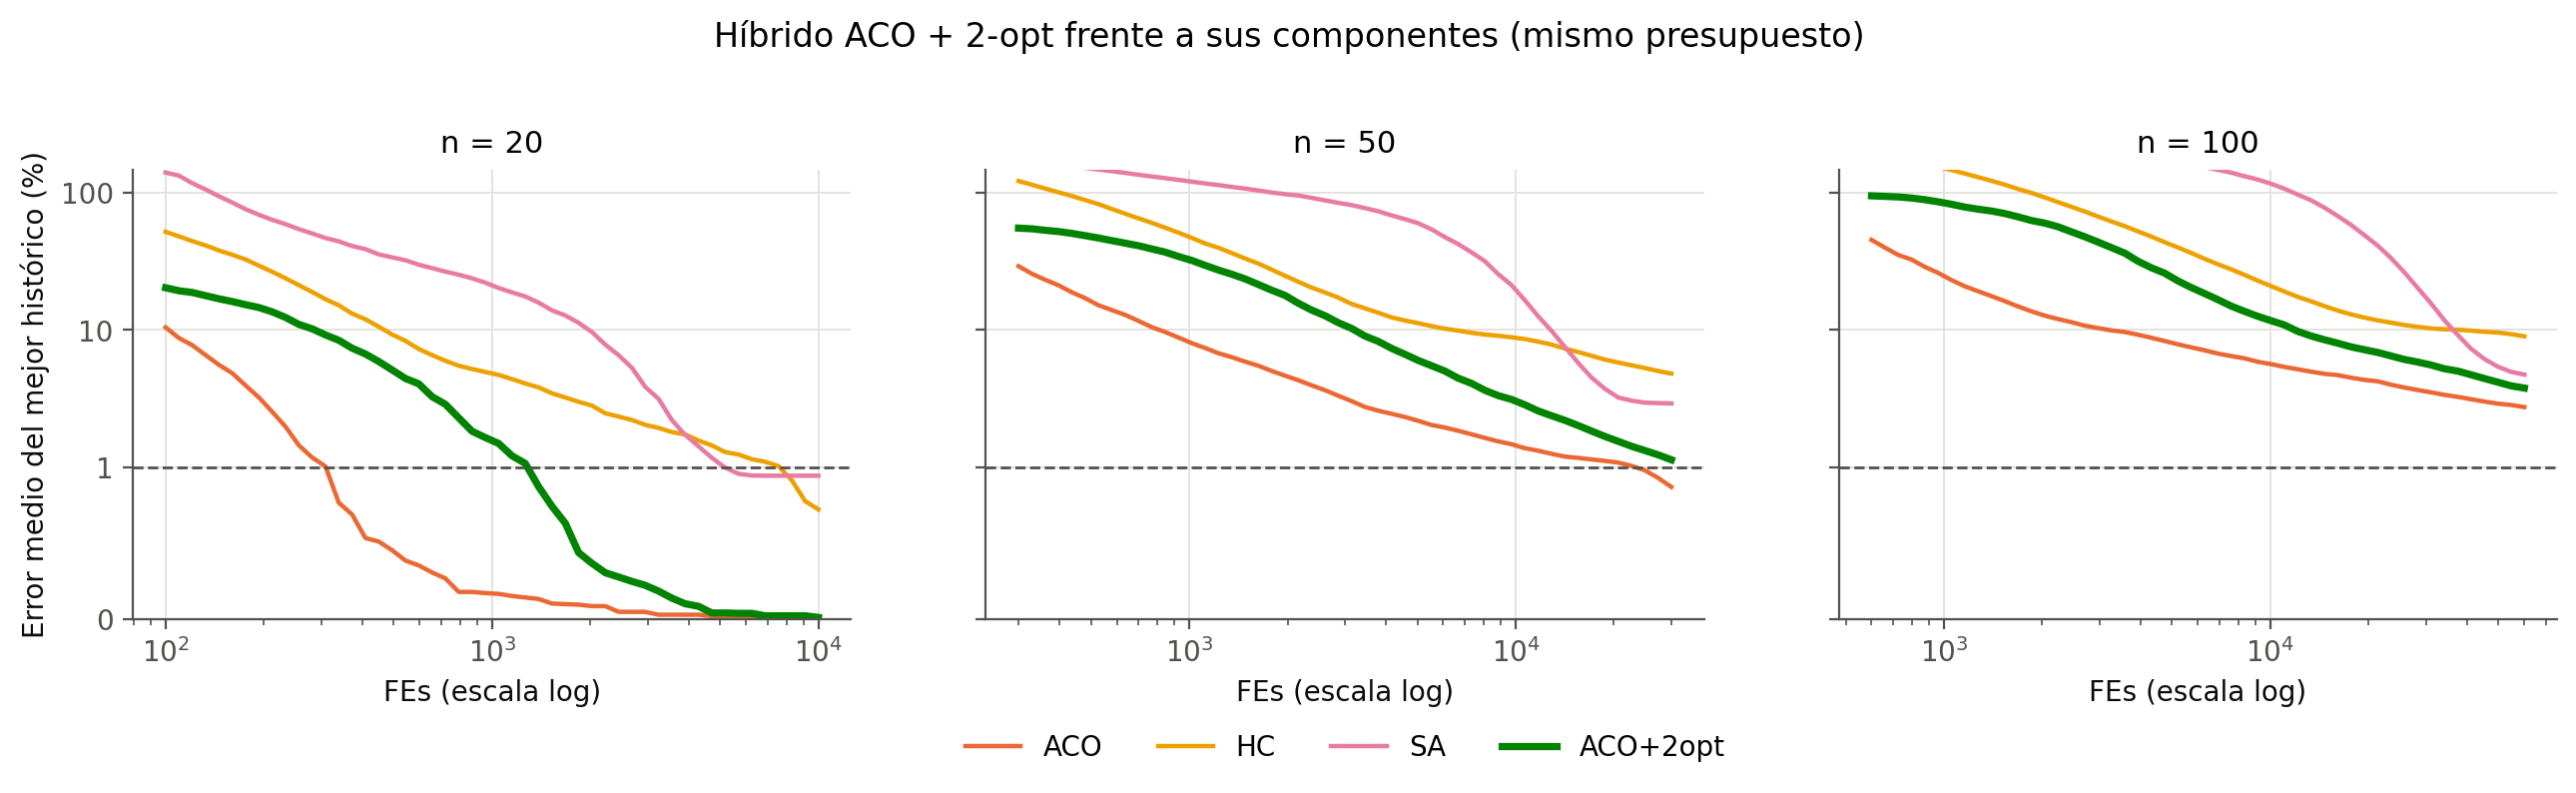
\includegraphics[width=\linewidth]{fig6_hibrido.png}
\caption{Error medio del mejor histórico: híbrido (línea gruesa) frente a ACO, HC y SA.}
\end{figure}

\begin{respuesta}[{¿La hibridación ofrece una mejora estadísticamente relevante?}]
\textbf{Frente a HC y SA, sí}: con $n=50$ y $n=100$ el híbrido gana en el 92--96\,\% de las corridas contra HC y en el 65--74\,\% contra SA ($p<10^{-4}$).
\textbf{Frente a ACO puro, no}: con $n=20$ empatan ($p=0{,}31$), y con $n=50$ y $n=100$ el ACO puro es \emph{mejor} (error mediano 0{,}66 vs 1{,}03\,\% y 2{,}66 vs 3{,}59\,\%; $p<0{,}01$).

\textbf{¿Por qué?} Con presupuesto fijo en \FEs, cada iteración del híbrido gasta $n$ \FEs\ en hormigas \emph{más} $5n$ en búsqueda local. Con $n=100$ eso es 600 \FEs\ por iteración:
la colonia solo alcanza $\approx100$ iteraciones en vez de 600, y la feromona aprende mucho menos. La búsqueda local es barata en \emph{tiempo}
(el híbrido tarda 0{,}96\,s frente a 5{,}2\,s del ACO con $n=100$), pero cara en \emph{evaluaciones}.

\textbf{Conclusión:} hibridar no mejora automáticamente; hay que balancear cuánto presupuesto va a explorar (colonia) y cuánto a explotar (búsqueda local).
Mejoras posibles: aplicar 2-opt solo en las últimas iteraciones, con menos pasos (p.\,ej. $n$ en lugar de $5n$), o usar listas de vecinos cercanos para proponer movimientos más prometedores.
Si el criterio de parada fuera el \emph{tiempo} y no las \FEs, el híbrido probablemente ganaría, porque cada evaluación suya es mucho más barata.
\end{respuesta}

% =====================================================================
\section{Cómo ejecutar todo y qué entregar}\label{sec:ejecutar}
% =====================================================================
\begin{lstlisting}[language=bash]
pip install -r requirements.txt
python -m pytest pruebas -q                                        # pruebas
python experimentos/piloto.py                                      # fase piloto (opcional)
python ejecutar_experimentos.py --config configuracion.json        # 2700 corridas (~30 min, 2 procesos)
python experimentos/analizar_resultados.py --config configuracion.json   # tablas y figuras
python experimentos/tablas_guia.py                                 # tablas LaTeX de esta guía
\end{lstlisting}

\textbf{Lista de verificación de la entrega} (sección ``Productos de entrega'' del taller):
\begin{center}\small
\begin{tabular}{>{\raggedright}p{5.2cm}>{\raggedright\arraybackslash}p{9.6cm}}
\toprule
Pedido & Dónde está \\
\midrule
1. \texttt{src/} implementación modular & 5 algoritmos + híbrido + \texttt{tsp.py}, \texttt{vecindad.py}, \texttt{interfaz.py}\\
2. \texttt{experimentos/} & \texttt{piloto.py}, \texttt{analizar\_resultados.py}, \texttt{tablas\_guia.py} y \texttt{ejecutar\_experimentos.py} en la raíz\\
3. \texttt{resultados/} & \texttt{ejecuciones.csv}, \texttt{corridas.jsonl} y todas las tablas resumidas\\
4. \texttt{figuras/} & PNG y PDF con título, unidades y leyenda\\
5. \texttt{informe.pdf} (máx.\ 8 páginas) & carpeta \texttt{informe/}\\
6. \texttt{README.md} & instalación, dependencias, ejecución, semillas, estructura\\
7. \texttt{requirements.txt} & versiones exactas\\
\bottomrule
\end{tabular}
\end{center}

% =====================================================================
\section*{Glosario rápido}
\addcontentsline{toc}{section}{Glosario rápido}
\begin{description}[leftmargin=2.8cm,style=nextline]
\item[FE] Una evaluación de la función objetivo (consultar la longitud de una ruta candidata).
\item[Presupuesto] Número máximo de \FEs\ que puede gastar un algoritmo en una corrida.
\item[Permutación] Un orden de las $n$ ciudades en el que cada una aparece exactamente una vez.
\item[Vecindad 2-opt] Rutas que se obtienen invirtiendo un tramo; elimina cruces.
\item[Óptimo local] Ruta que no se puede mejorar con un solo movimiento de la vecindad.
\item[Exploración] Buscar en regiones nuevas. \textbf{Explotación}: afinar cerca de lo que ya es bueno.
\item[Elitismo] Pasar los mejores individuos sin cambios a la siguiente generación.
\item[Feromona] Memoria colectiva de ACO sobre qué aristas han estado en buenas rutas.
\item[Claves aleatorias] Codificar una ruta como un vector real cuyo orden da la permutación.
\item[Metropolis] Regla de SA: aceptar un empeoramiento $\Delta$ con probabilidad $e^{-\Delta/T}$.
\item[$f^\ast$] Mejor longitud conocida de la instancia (aquí: la mejor encontrada por cualquier algoritmo).
\item[RIC] Rango intercuartílico, $Q_3-Q_1$: ancho de la mitad central de los datos.
\item[Friedman] Prueba no paramétrica que compara $k$ algoritmos con datos emparejados usando rangos.
\item[Holm] Corrección que ajusta los valores $p$ cuando se hacen muchas comparaciones.
\item[W de Kendall] Tamaño del efecto de Friedman (0: sin acuerdo; 1: mismo orden siempre).
\end{description}

\end{document}

